%\documentclass[3p,twocolumn]{elsarticle}
\documentclass[review]{elsarticle}
\usepackage{graphicx}
\usepackage[export]{adjustbox}%for left right graphic adjust
\usepackage{amsmath}
\usepackage{float}
\usepackage{overpic}
\usepackage{contour}
\usepackage{color}
\usepackage{comment}
\graphicspath{ {images/} }

\usepackage[T1]{fontenc}
%\usepackage[utf8]{inputenc}
\usepackage{lineno,hyperref}
\modulolinenumbers[5]

\journal{Journal of \LaTeX\ Templates}

%%%%%%%%%%%%%%%%%%%%%%%
%% Elsevier bibliography styles
%%%%%%%%%%%%%%%%%%%%%%%
%% To change the style, put a % in front of the second line of the current style and
%% remove the % from the second line of the style you would like to use.
%%%%%%%%%%%%%%%%%%%%%%%

%% Numbered
%\bibliographystyle{model1-num-names}

%% Numbered without titles
%\bibliographystyle{model1a-num-names}

%% Harvard
%\bibliographystyle{model2-names.bst}\biboptions{authoryear}

%% Vancouver numbered
%\usepackage{numcompress}\bibliographystyle{model3-num-names}

%% Vancouver name/year
%\usepackage{numcompress}\bibliographystyle{model4-names}\biboptions{authoryear}

%% APA style
%\bibliographystyle{model5-names}\biboptions{authoryear}

%% AMA style
%\usepackage{numcompress}\bibliographystyle{model6-num-names}

%% `Elsevier LaTeX' style
\bibliographystyle{elsarticle-num}
%%%%%%%%%%%%%%%%%%%%%%%

\begin{document}

\begin{frontmatter}

\title{Extending the Dynamic Range of Electronics in a Time Projection Chamber}

%% Group authors per affiliation:
%\author{Elsevier\fnref{myfootnote}}
%\address{Radarweg 29, Amsterdam}
%\fntext[myfootnote]{Since 1880.}

%% or include affiliations in footnotes:
\author[nscl,msu]{J. Estee}
\author[nscl,msu]{W.G. Lynch}
\author[nscl,msu]{J. Barney}
\author[nscl,msu]{G. Cerizza}
\author[kor]{B. Hong}
\author[riken]{T. Isobe}
\author[nscl]{G. Jhang}
\author[kyoto]{M. Kaneko}
\author[riken]{M. Kurata-Nishimura}
\author[krakow]{P. Lasko}
\author[kor]{J. W. Lee}
\author[krakow]{J. \L ukasik}
\author[a&m]{A.B. McIntosh}
\author[kyoto]{T. Murakami}
\author[krakow]{P. Paw\l owski}
\author[poland]{K. Pelczar}
\author[nscl]{C. Santamaria}
\author[riken]{D. Suzuki}
\author[nscl]{M. B. Tsang}
\author[china1,china2]{R. Wang}
\author[a&m]{S.J. Yennello}
\author[tsing]{Y. Zhang}
\author[]{and the S$\pi$RIT collaboration}

\address[nscl]{National Superconducting Cyclotron Laboratory, East Lansing, Michigan, 48824, USA}
\address[msu]{Department of Physics and Astronomy, Michigan State University, East Lansing, Michigan, 48824, USA }
\address[kor]{Department of Physics, Korea University, Seoul 136-703, Republic of Korea }
\address[riken]{RIKEN Nishina Center, Hirosawa 2-1, Wako, Saitama 351‐0198, Japan }
\address[kyoto]{Department of Physics, Kyoto University, Kita-shirakawa, Kyoto 606-8502, Japan }
\address[krakow]{Institute of Nuclear Physics PAN, ul. Radzikowskiego 15231-342 Krak\'{o}w, Poland}
\address[a&m]{Cyclotron Institute, Texas A$\&$M University, College Station, TX 77843, USA }
\address[tsing]{Department of Physics, Tsinghua University, Beijing 100084, P. R. China}
\address[poland]{Faculty of Physics, Astronomy and Applied Computer Science, Jagiellonian University, ul. Go\l \k{e}bia 24, 31-007 Krak\'{o}w}
\address[china1]{State Key Laboratory of Radiation Medicine and Protection, School of Radiation Medicine and Protection, Soochow University, Suzhou 215123, China}
\address[china2]{Collaborative Innovation Center of Radiological Medicine of Jiangsu Higher Education Institutions, Suzhou 215123, China}



\begin{abstract}

When Time Projection Chambers (TPCs) are used in low to intermediate heavy ion collisions, the mass and momentum range covered by the emitted particles cover a wide range in energy losses. Many TPC readout electronics currently only have a single gain output with a fixed dynamic range. In a recent set of experiments using the SAMURAI Pion-Reconstruction and Ion-Tracker (S$\pi$RIT) TPC, it was important to simultaneously measure relativistic pions and heavy ion tracks from the same collisions. As a tracks energy loss is collected and multiplied by the anode wires, a distribution of image charges are induced on the TPC read out pads. If the avalanche on a wire is large enough, the charge collected on a pad will saturate the electronics, though only for pads directly underneath the avalanche; pads further away in the distribution will not be saturated. Using these unsaturated pads and the known distribution function, we can estimate the saturated pads, increasing the dynamic range by a factor of 5.

\end{abstract}

\begin{keyword}
\texttt{elsarticle.cls}\sep \LaTeX\sep Elsevier \sep template
\MSC[2010] 00-01\sep  99-00
\end{keyword}

\end{frontmatter}

\linenumbers

\section{Introduction} 
 Charged particles emitted in low to intermediate energy nuclear collisions cover a large range in energy losses from very small energy losses, for minimum ionizing particles, to much higher energy losses, for slower moving, heavy fragments. Figure \ref{fig:intro} shows the range of momenta typically observed in intermediate energy collisions, around 300 MeVA, and the energy loss range involved.  
 
  Measuring the full range in energy losses have motivated the development of large dynamic range electronics, which are able to switch between high and low gains covering a very large dynamic range; however, many current Time Projection Chambers (TPCs) readout electronics have a single gain output, presenting a problem for the readout of such devices.
 
 Several techniques have been employed to increase the dynamic range for energy losses in TPCs. One solution is to lower the electronics gain or the avalanche gas gain in certain regions of the TPC, increasing the dynamic range. In the EOS TPC \cite{eos}, a larger dynamic range was achieved by lowering the voltage on selected anode wires, decreasing the gas amplification on those wires while in the prototype Active Target TPC (PAT-TPC) and AT-TPC an equivalent reduction in gain was achieved by lowering the electronics gain for some of the readout channels.  By dedicating regions of lower gain in the TPC one is able to measure more strongly ionizing particles, but for these regions of lower gain the weakly ionizing particle's signals are to small to be measured and we lose information for determining the momentum. 
 
 The need to measure the full range in energy losses has motivated the development of large dynamic range electronics, which are able to switch between high and low gains [Pollacco, private communications] covering a very large dynamic range. However, many current TPCs have a single fixed gain output, presenting a problem for the analysis of data taken with the readout of such devices.

 These strategies have drawbacks in applications where the experiment's requirements cannot accept the associated degradation in the dE/dx resolution, or the momentum resolution. Finding the solution to this problem has motivated the development of software based analysis that will extend the dynamical range of TPCs; we illustrate an alternate approach to expand the dynamic range within the context of a standard multi-wire TPC, without the need of extra hardware or dedicating regions of lower gain. 
 
 Many TPC readout electronics have a single gain output with a dynamic range (defined the ratio of the maximum signal to the electronic noise) of no more than 1000:1. In our case the maximum signal to noise was about 700:1. We required the smallest signal of minimum ionizing particles (m.i.p.) to be 30:1, setting the dynamic range to be 23 times m.i.p. Figure \ref{fig:intro} illustrates the range in momentum we expect to see saturation effects. The shaded region shows where 23 times that of the minimum ionizing pion signal where we could expect saturation to occur. While the pion's momentum range can fully be measured, without saturation effects, heavier particles would be harder to resolve in dE/dx at lower momentum.

 
 
\begin{figure}[H]
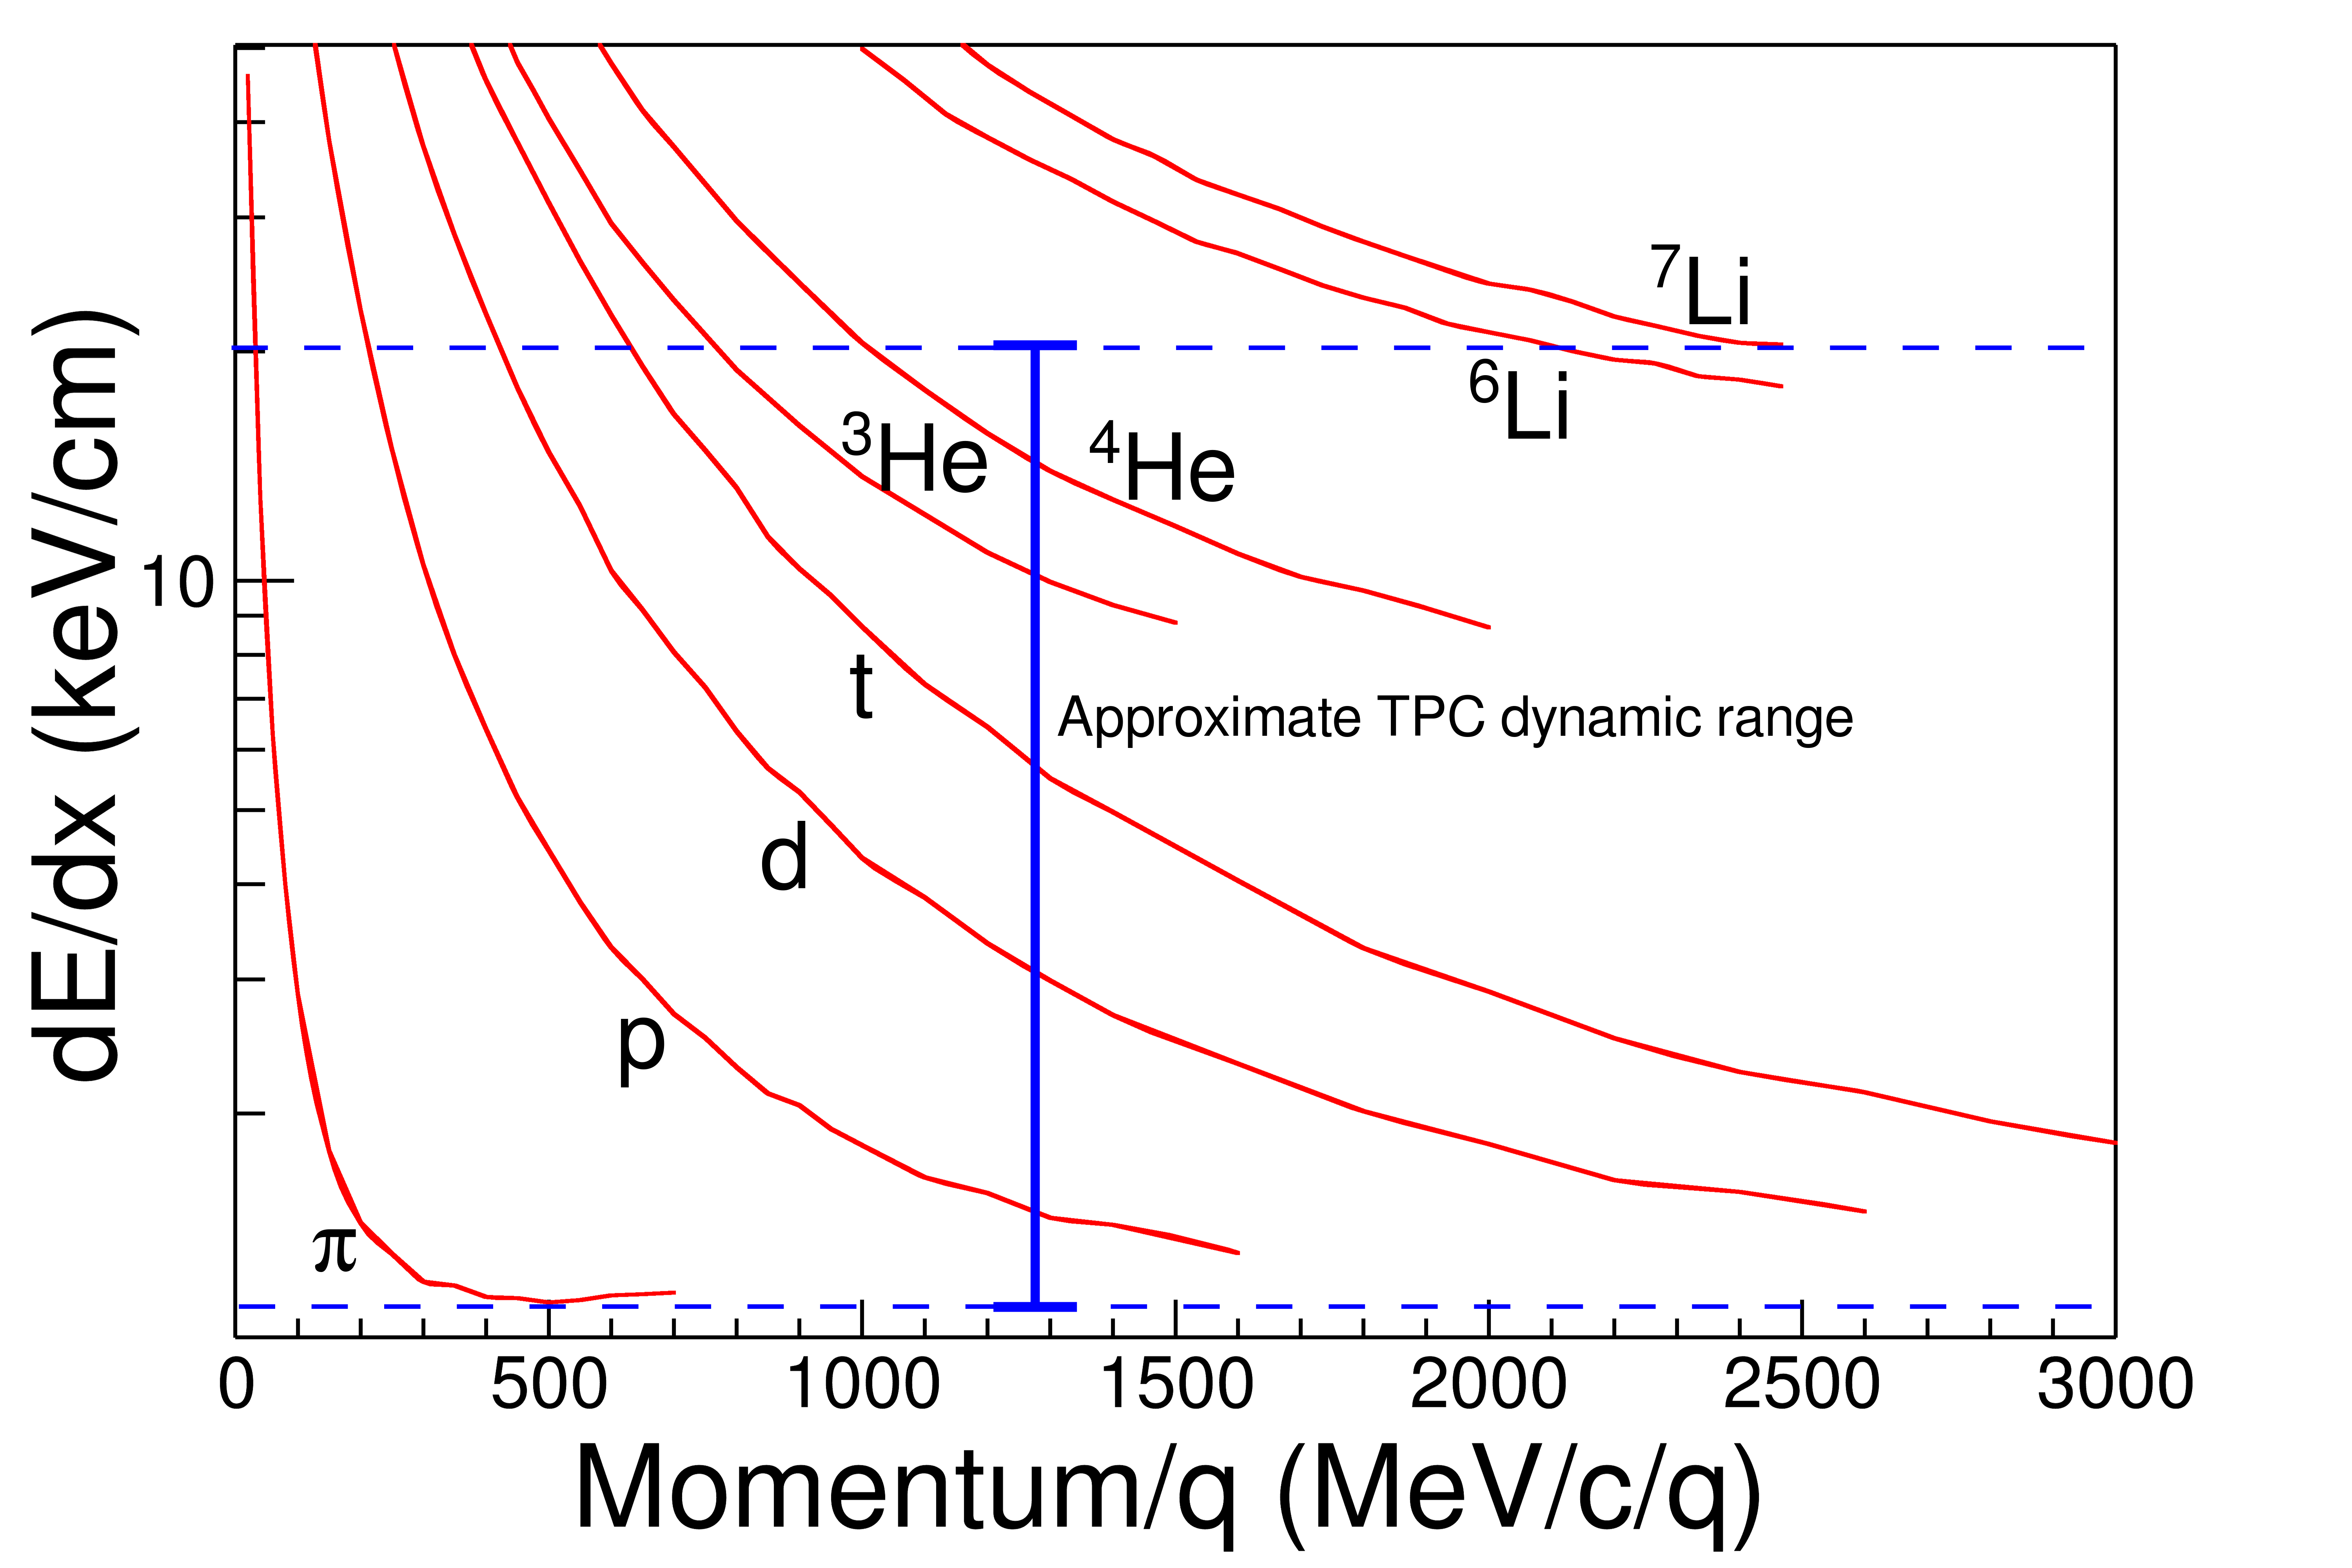
\includegraphics[width=\linewidth]{intrographic}
\caption{The expected dE/dx lines of different particles are given in red as calculated by GEANT4. The approximate dynamic range of the TPC is shown for the gain setting used in the experiment. Anything outside of this region would be saturated to some degree.}
\label{fig:intro}
\end{figure}

\paragraph{1.1 TPC Overview}
We begin our discussion by describing some basic properties of the SAMURAI Pion Reconstruction and Ion-Tracker (S$\pi$RIT) TPC \citep{shane}. It is a rectangular TPC with 12,096 pads designed to constrain the density dependence of the nuclear symmetry energy at densities on the order of twice saturation density. In order to study central collisions of Sn isotopes at around 300 AMeV, the TPC was designed to identify isotopes up to Z=3 with the ability to detect low ionizing particles such as pions. 

 For the following discussion we have defined the +x axis to point to the left of the beam, the -y axis to point down into the drift volume, and the +z axis to point along the beam. 

\begin{figure}[H]
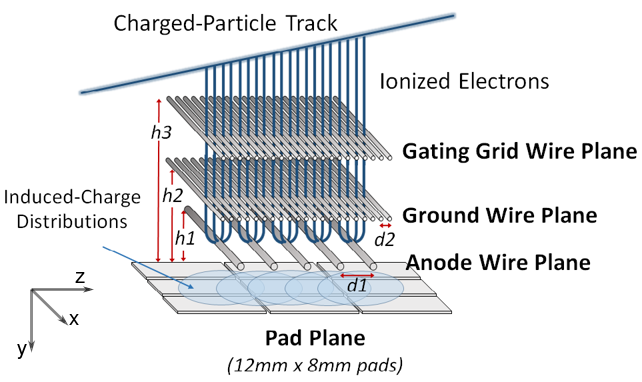
\includegraphics[width=\linewidth]{padwire}
\caption{Cartoon graphic showing the 3 wire planes and a section of the pad plane. h3 =14 mm, h2 = 8 mm, h1 = 4 mm, d2 = 1 mm, d1 = 4 mm. This graphic is inverted from the actual wire planes and pad plane to display the perspective easier.}
\label{fig:padwire}
\end{figure}

\paragraph{Pad plane} 
The S$\pi$RIT TPC pad plane is composed of a rectangular charge sensitive pads, each with an x dimension of of 8 mm wide, and a z dimension of 12 mm. These pads are arranged in a grid measuring 112 by 108 pads with a total area of 1344 mm x 864 mm.

\paragraph{Wire planes}
As illustrated in Figure \ref{fig:padwire}, the S$\pi$RIT TPC consists of three wire planes below the pad plane, with the wires aligned along the x-axis. The wire plane farthest from the pad plane (14 mm) operates as an ion-gate or a gating grid. Details on the gating grid can be found in \cite{suwat}. The middle wire plane (8 mm) is grounded. When the gating grid is open, electrons ionized by reaction products in the drift volume drift through both the gating grid and ground planes. 

Closest to the pad plane is the high voltage, anode wire plane (4 mm), consisting of 20 $\mu$m diameter wires spaced 4 mm apart. In the vicinity of these wires an avalanche occurs multiplying the secondary electrons drifting up from the drift volume, created from the track's energy loss in the detector gas. When these secondary electrons reach the anode wires, they are amplified on the order of 1000 times creating electron and ion pairs. It is the motion of these slow moving ions, as they drift away from the anode wires, that induces image charges on the read out pads above. The distribution of image charged on the pad plane is centered about the avalanche region on the wires and its width is fixed by the distance from the pad plane. 

The anode wires are sectioned off into 14 independent sections, each containing 26 wires; 12 sections were biased to 1460 V. This setting was optimized to ensure m.i.p. particles such as pions would have a signal to noise ratio of around 20:1. The two remaining sections were biased to 1214 V due to high current issues, reducing the gas gain by a factor of 10 times as compared to the other anode sections. As demonstrated by the EOS TPC \citep{eos}, lowering the anode wires effectively extended the dynamic range.  This gain reduction allowed for a direct validation of the success of the new method for extending the dynamic range presented here. 

\paragraph{Generic Electronics for TPCs}
Signals in the S$\pi$RIT TPC are amplified and digitized by the recently developed Generic Electronics for TPCs (GET) \cite{get}.  Short cables transmit the signals from the pads to the inputs of the AGET chips. Each AGET chip services 64 pads (63 pads are connected in our case), contains a pre-amplifier, and a Switched Capacitor Array (SCA), with a maximum of 512 time buckets with an adjustable sampling frequency of 1 to 100 MHz. Four AGET chips are mounted on one AsAd (ASIC and ADC) motherboard. The gain of each AGET can be configured as 0.12, 0.24, 1.0, or 10 pC over the whole dynamic range, and the ADCs on each AsAd board provides 12 bit resolution. The peaking times of the shaping amplifiers can be set to 69, 117, 232, 501, 720, or 1014 ns. In this experiment, the gain was set to the highest setting, 0.12 pC, the peaking time 117 ns, and the sampling frequency 25 MHz (resulting in 40 ns time buckets). The AGET 2.0, ASAD 2.1, and COBO 1.0 firmware versions were used. The variations in the electronics were calibrated by measuring the response of each channel to an injected reference pulse, covering the full dynamic range of each channel. 

\paragraph{Analysis Software}
The S$\pi$RITROOT software is modular tasked based code based on the FAIRROOT package written in C++ \cite{fairroot}. The main tasks in the S$\pi$RITROOT software reconstruction are:
\begin{itemize}
  \item Decoder task
  \item Pulse Shape Algorithm (PSA Task)
  \item Helix Track Finding Algorithm
  \item Clustering Algorithm
  \item Track Fitting (Momentum determination by the GENFIT package)
  \item Vertex Fitting (RAVE package)
\end{itemize}

The decoder task converts the binary data file into a container class which maps the electronics channels into the corresponding pads and (x,z) coordinates. 

There may be several pulses in a pad coming from two tracks passing under the same pad separated  by arrival time. Using an expected pulse shape the PSA task fits the signal pulses within a pad, giving the arrival time of the drifted electrons from each particular track. The height of the fitted pulse is proportional to the total charge of that event, Q and the y-coordinate is calculated as $y = v\cdot t_0$ where $v$ is the drift velocity and $t_0$ the arrival time. Combining the information from these first two tasks, (x,y,z,Q), we construct what is called a "hit". 

 The Helix Track Finding Algorithm finds the collection of hits belonging to one track out of all the hits in an event. The hits within a track are then reduced into clusters. A cluster's position is the average position of the hits within a cluster, with the total charge of the cluster being the sum of the hits charges. 
 
 A tracks average position is estimated by the cluster's average position. The clusters are then fitted in the GENFIT track fitting package \cite{genfit}, giving the final momentum of the track. A final vertex of the event is fitted from all tracks using the package RAVE \cite{rave}. 
 

\paragraph{Definition of clustering}

A brief description of the method of clustering is illustrated in Figure \ref{fig:topview}. It is impractical to cluster in both the x and z-axis and we only cluster the hits along one axis. The three clusters at the bottom of Figure \ref{fig:topview} are clustered along the x-axis and the upper three are along the z-axis, as shown by the bolded pads for one of the clusters in each direction.

 The clustering direction depends on the angle  of the track with respects to the x-axis, defined as $\theta$. For example, a track going along the z-axis the crossing angle is defined as $90^{\circ}$, and a track going along the x-axis defined as $0^{\circ}$. In the case that the crossing angle is $45^{\circ} < \theta \leq 90^{\circ} $ the clustering direction is along the x-axis. For $0^{\circ} < \theta \leq 45^{\circ}$ it is along the z-axis. 

 The position along the clustering direction is calculated by weighting the individual hit's positions by their charges $q_i$ and getting the mean value. The other direction is set to the center of the pad. For example if we are clustering along the x-axis for a cluster, the z-position is set to the center of the pad in the z-direction and vice versa. 

Clustering in this way gives us better position resolution for calculating the position of each cluster. You could imagine if we calculated the clusters only along the x-axis for tracks with $\theta \approx 0^{\circ}$ the x-position is not well defined. By clustering in the direction most perpendicular to the track, we get a better position resolution.



\begin{figure}[H]
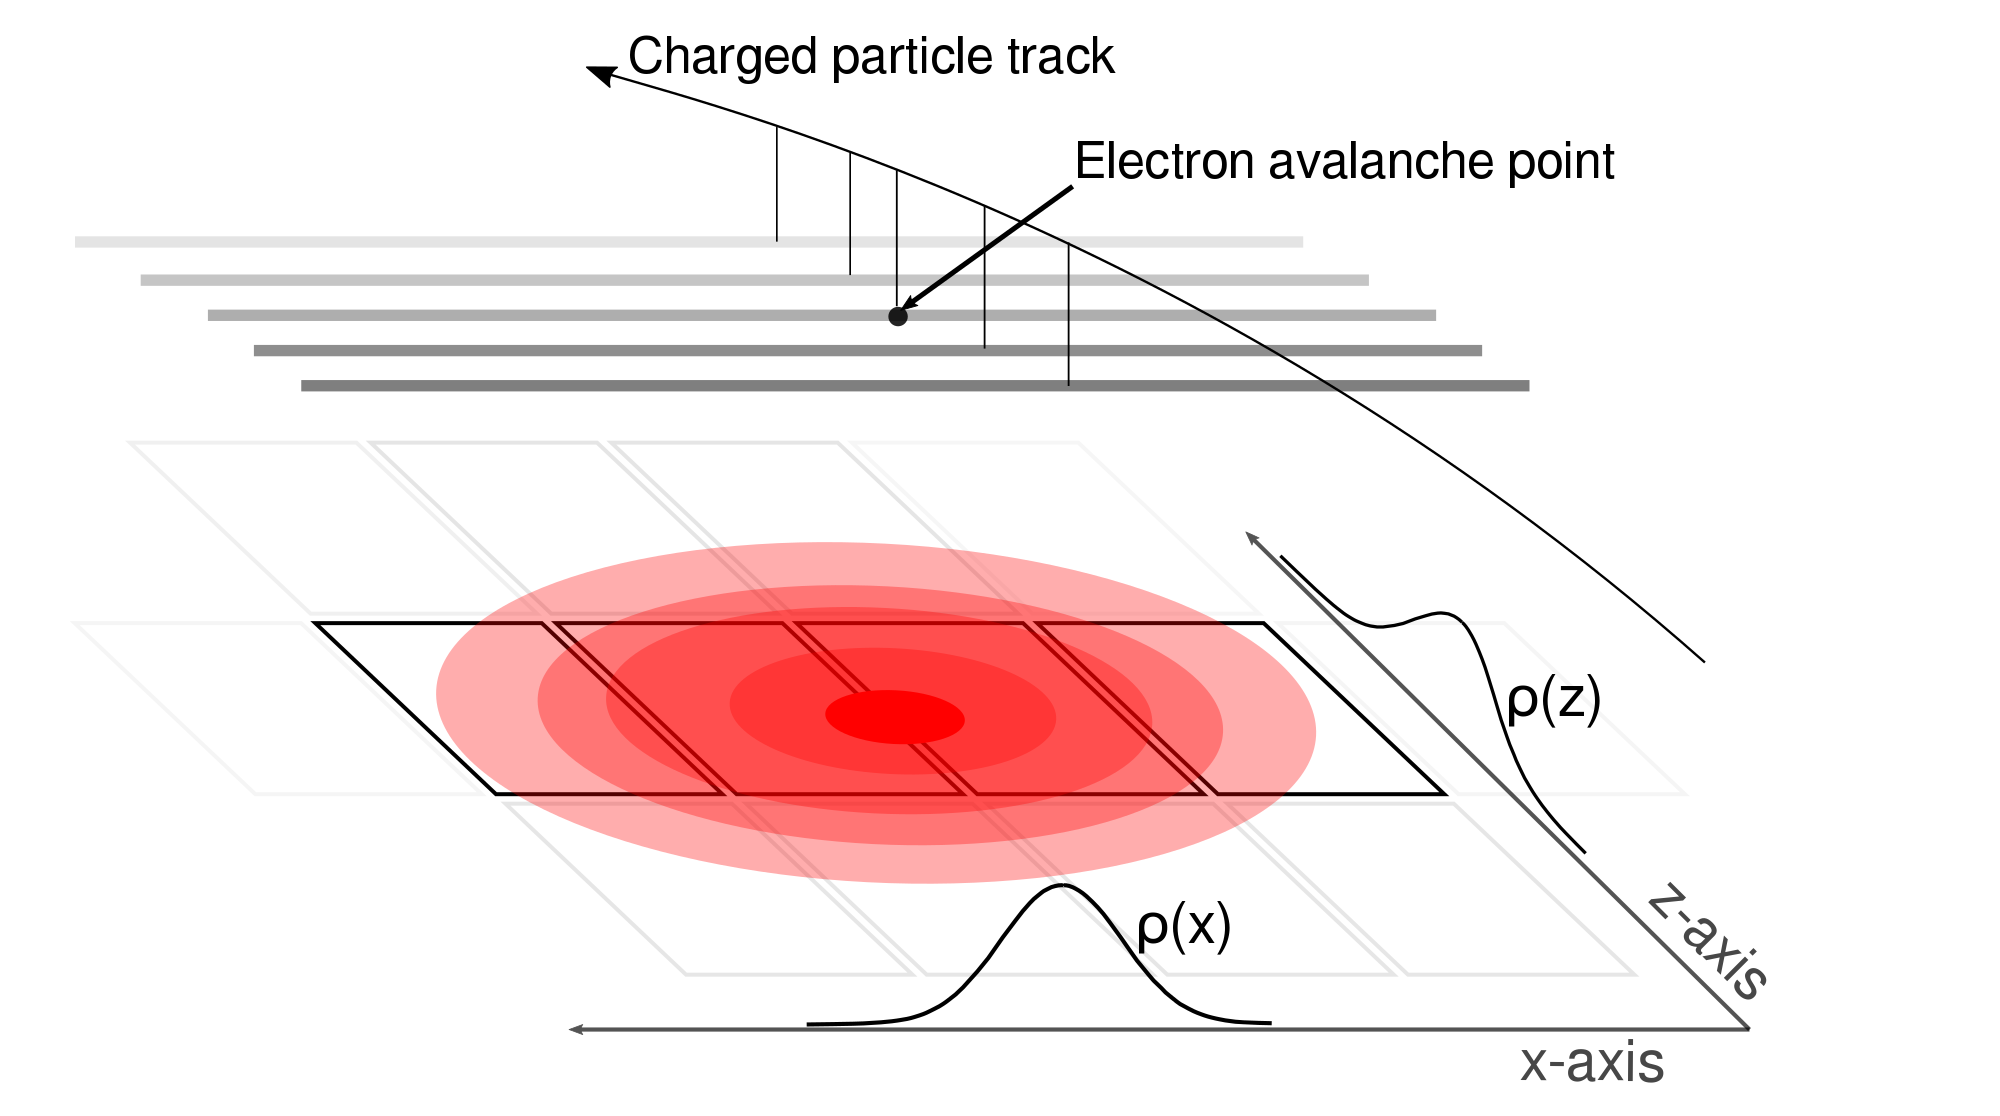
\includegraphics[width=\linewidth]{padsat_Large}
\caption{A cartoon illustration of the charge distribution resulting from an electron avalanche on one wire and the projections of the distribution onto the two axis $\rho(x)$ onto the x-axis and $\rho(z)$ onto the z-axis. The orientation of the wire planes is flipped upside down to display the perspective better.}
\label{fig:prf}
\end{figure}

\section{Pad Response Function}
As illustrated in Figure \ref{fig:prf} the distribution resulting from an electron avalanche is 2-dimensional, with the charge observed on each pad being the integral of that distribution over the pad's dimensions; also called the Pad Response Function (PRF). The projection onto the x and z-axis of this distribution is shown as $\rho(x)$ and $\rho(z)$. 

In this example the clustering direction would be along the x-axis, as illustrated by the bolded pads. By choosing to clustering only in one direction, we have not included the charge in adjacent pads along the z-axis resulting from the tails of $\rho(z)$. Therefore the charge not included in the the bolded pads will be included in adjacent clusters, introducing small correlations in charge between neighboring clusters. 

\begin{figure}[H]
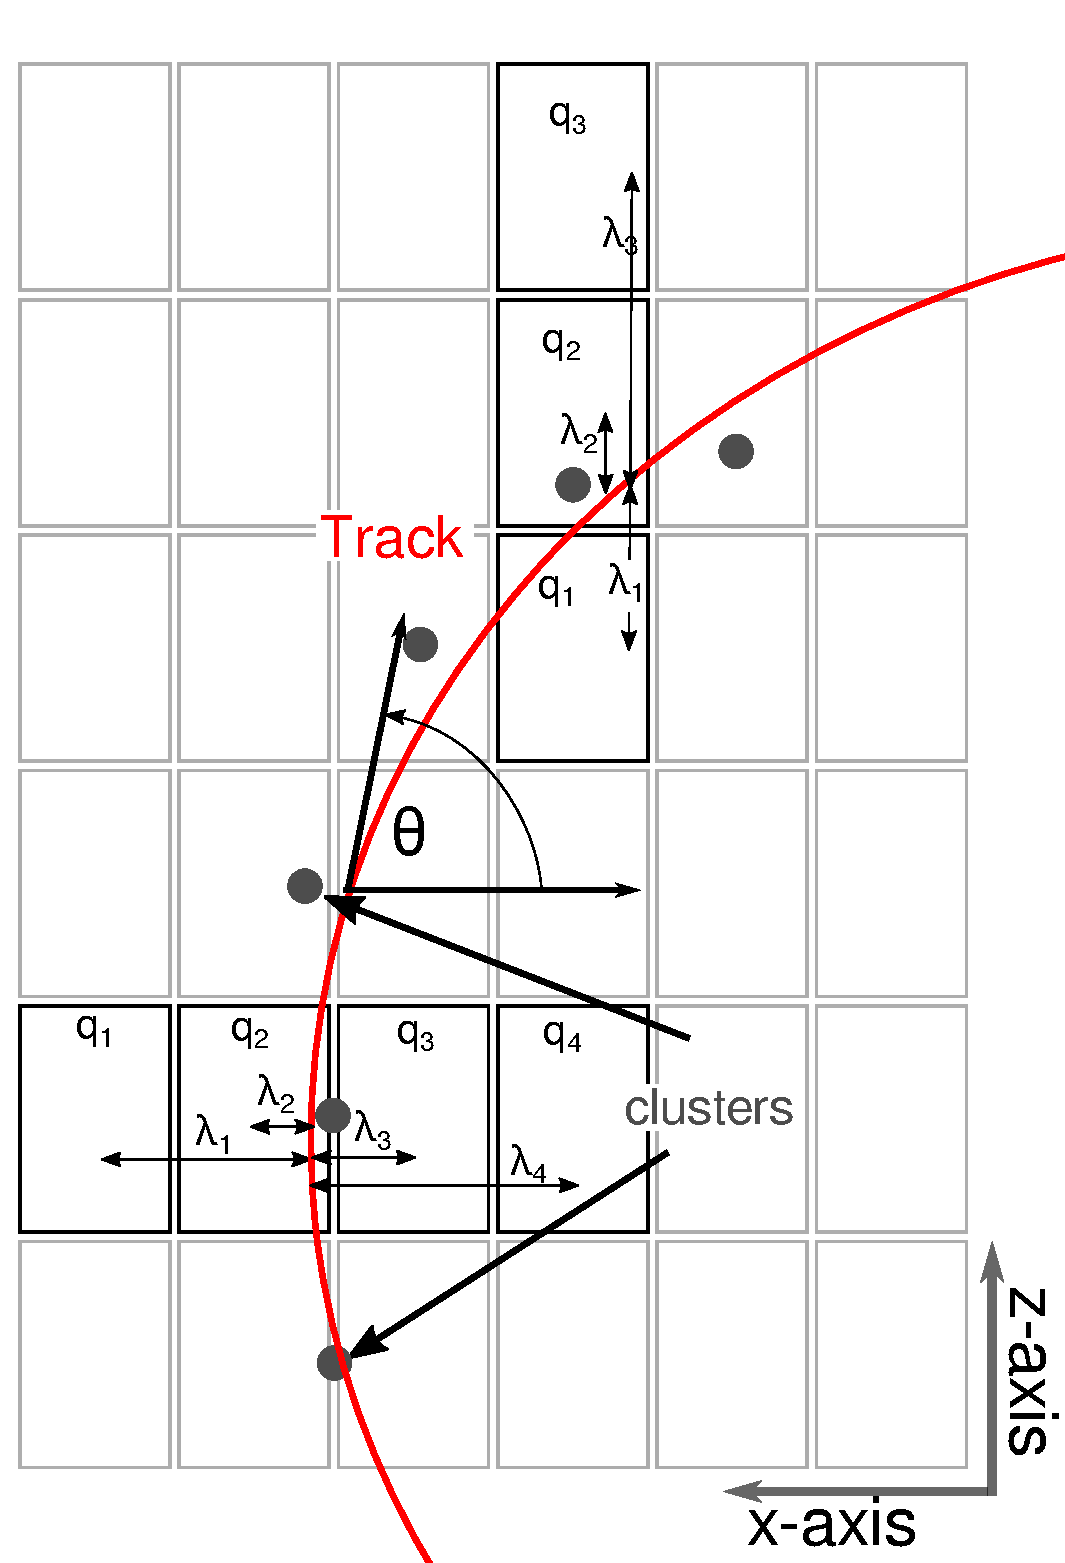
\includegraphics[scale=.5]{top_view_helix_ext.pdf}
\caption{Cartoon graphic of a top down view of a fit to a track passing through several pads. The bolded pads and the charges $q_i$ represent the hits belonging to that pad and the clusters of the track representing the average position of the track. The three clusters at the bottom are clustered in the x-direction and for the upper three clustered in the z-direction. The estimate of the position of the avalanche is given by the track fit and the position from the center to each pad to the $\bar{x}$ position is given as $\lambda_i$.}
\label{fig:topview}
\end{figure}

\paragraph{Gatti Pad Response Function}
Gatti \cite{gatti} expressed a semi-empirical equation for the charge distribution in a simple multi-wire TPC such as that found in the S$\pi$RIT TPC. Given in Eq. \ref{eq:gatti}, the function depends only on the width of a pad (w), height of the anode plane to the pad plane (h), and the distance of the pad center to the avalanche point $\lambda$. It is a single parameter equation where the two parameters $K_1 = \frac{K_{2}\sqrt{K_3}}{4 atan(\sqrt{K_3})}$ and $K_2 = \frac{\pi}{2}\left(1-\frac{\sqrt{K_{3}}}{2}\right)$ depend on the parameter $K_3$, which is a function of the ratio of the anode wire diameter to the height of the anode wires to the pad plane. $K_3$ can be looked up in a graph in \cite{blumrol} and \citep{gatti}.

\begin{equation}\label{eq:gatti}
\begin{split}
PRF_{gatti}(\lambda)
& = \frac{K_{1}}{K_{2}\sqrt{K_{3}}}\bigl[arctan(\sqrt{K_{3}}tanh\bigl[K_{2}\bigl(\frac{\lambda}{h}+\frac{w}{2h}\bigr)\bigr]) \\
& - arctan(\sqrt{K_{3}}tanh\bigl[K_{2}\bigl(\frac{\lambda}{h}-\frac{w}{2h}\bigr)\bigr])\bigr] \\
\end{split}
\end{equation}

\paragraph{Experimental PRF}

The correlations we introduced by only clustering along one direction do not play a significant role in the particle identification, but cause deviations from the expected Gatti distribution. Also, analytic PRFs only exist for classical multi-wire TPCs. For these reasons it is useful to experimentally measure the PRF and fit it with some empirical function, typically a Gaussian, to describe its behavior. 

As shown in Figure \ref{fig:topview}, we postulate that the PRF is a function of the total charge deposited in a cluster $Q = \sum_i q_i$ and the difference in position of the center of the $i^{th}$ pad, $x_i$, to the mean position $\bar{x} = \sum_i x_i q_i/Q$, which we call $\lambda_i = x_i-\bar{x}$. The PRF is simply defined as the charge fraction of each pad as a function of $\lambda$, Equation \ref{eq:prf}. 

\begin{equation}\label{eq:prf}
PRF(\lambda_i) = \frac{q_i(\lambda_i)}{Q}
\end{equation}

Averaging over many events in the experimental data, the resulting PRF for the S$\pi$RIT TPC is shown in Figure \ref{fig:expprf}. Here we see the deviations from the expected analytic Gatti distribution where as fitting with a two parameter Gaussian function describes the data better. With the two parameters being the normal coefficient,$N_0$, sigma $\sigma$, and with a mean value assumed to be 0 as given in Equation \ref{eq:gaus}.

\begin{equation}\label{eq:gaus}
PRF_{gaus}(\lambda) = N_0 e^\frac{-\lambda^2}{2\sigma^2}
\end{equation}

\begin{figure}[H]
\begin{overpic}[width=\linewidth]{expprf}
\put(61,55){\contour{white}{ PRF${}_{gaus}(\lambda)$ eq. \ref{eq:gaus}  }}
\put(61,49){\contour{white}{ PRF${}_{gatti}(\lambda)$ eq. \ref{eq:gatti} }}
\end{overpic}
\caption{Experimental pad response function of many events for a crossing angle of $85^{\circ} < \theta \leq 90^{\circ}$.  }
\label{fig:expprf}
\end{figure}

\section{PRF vs crossing angle}
The shape of the PRF depends on the crossing angle \citep{gatti}. As plotted in Figure \ref{fig:prfangle} is the PRF of a $\pi^-$ tracks vs the crossing angle $\theta$. One can see the PRF gets wider going from  $90^{\circ}$ to $45^{\circ}$. Once could imagine if we did not switch clustering directions the PRF would become wider until it was a uniform distribution and there was no position resolution. Since we switch the clustering direction from x to z at $45^{\circ}$, the opposite trend is seen where the PRF becomes narrower going from $45^{\circ}$ to $0^{\circ}$.

\begin{figure}[H]
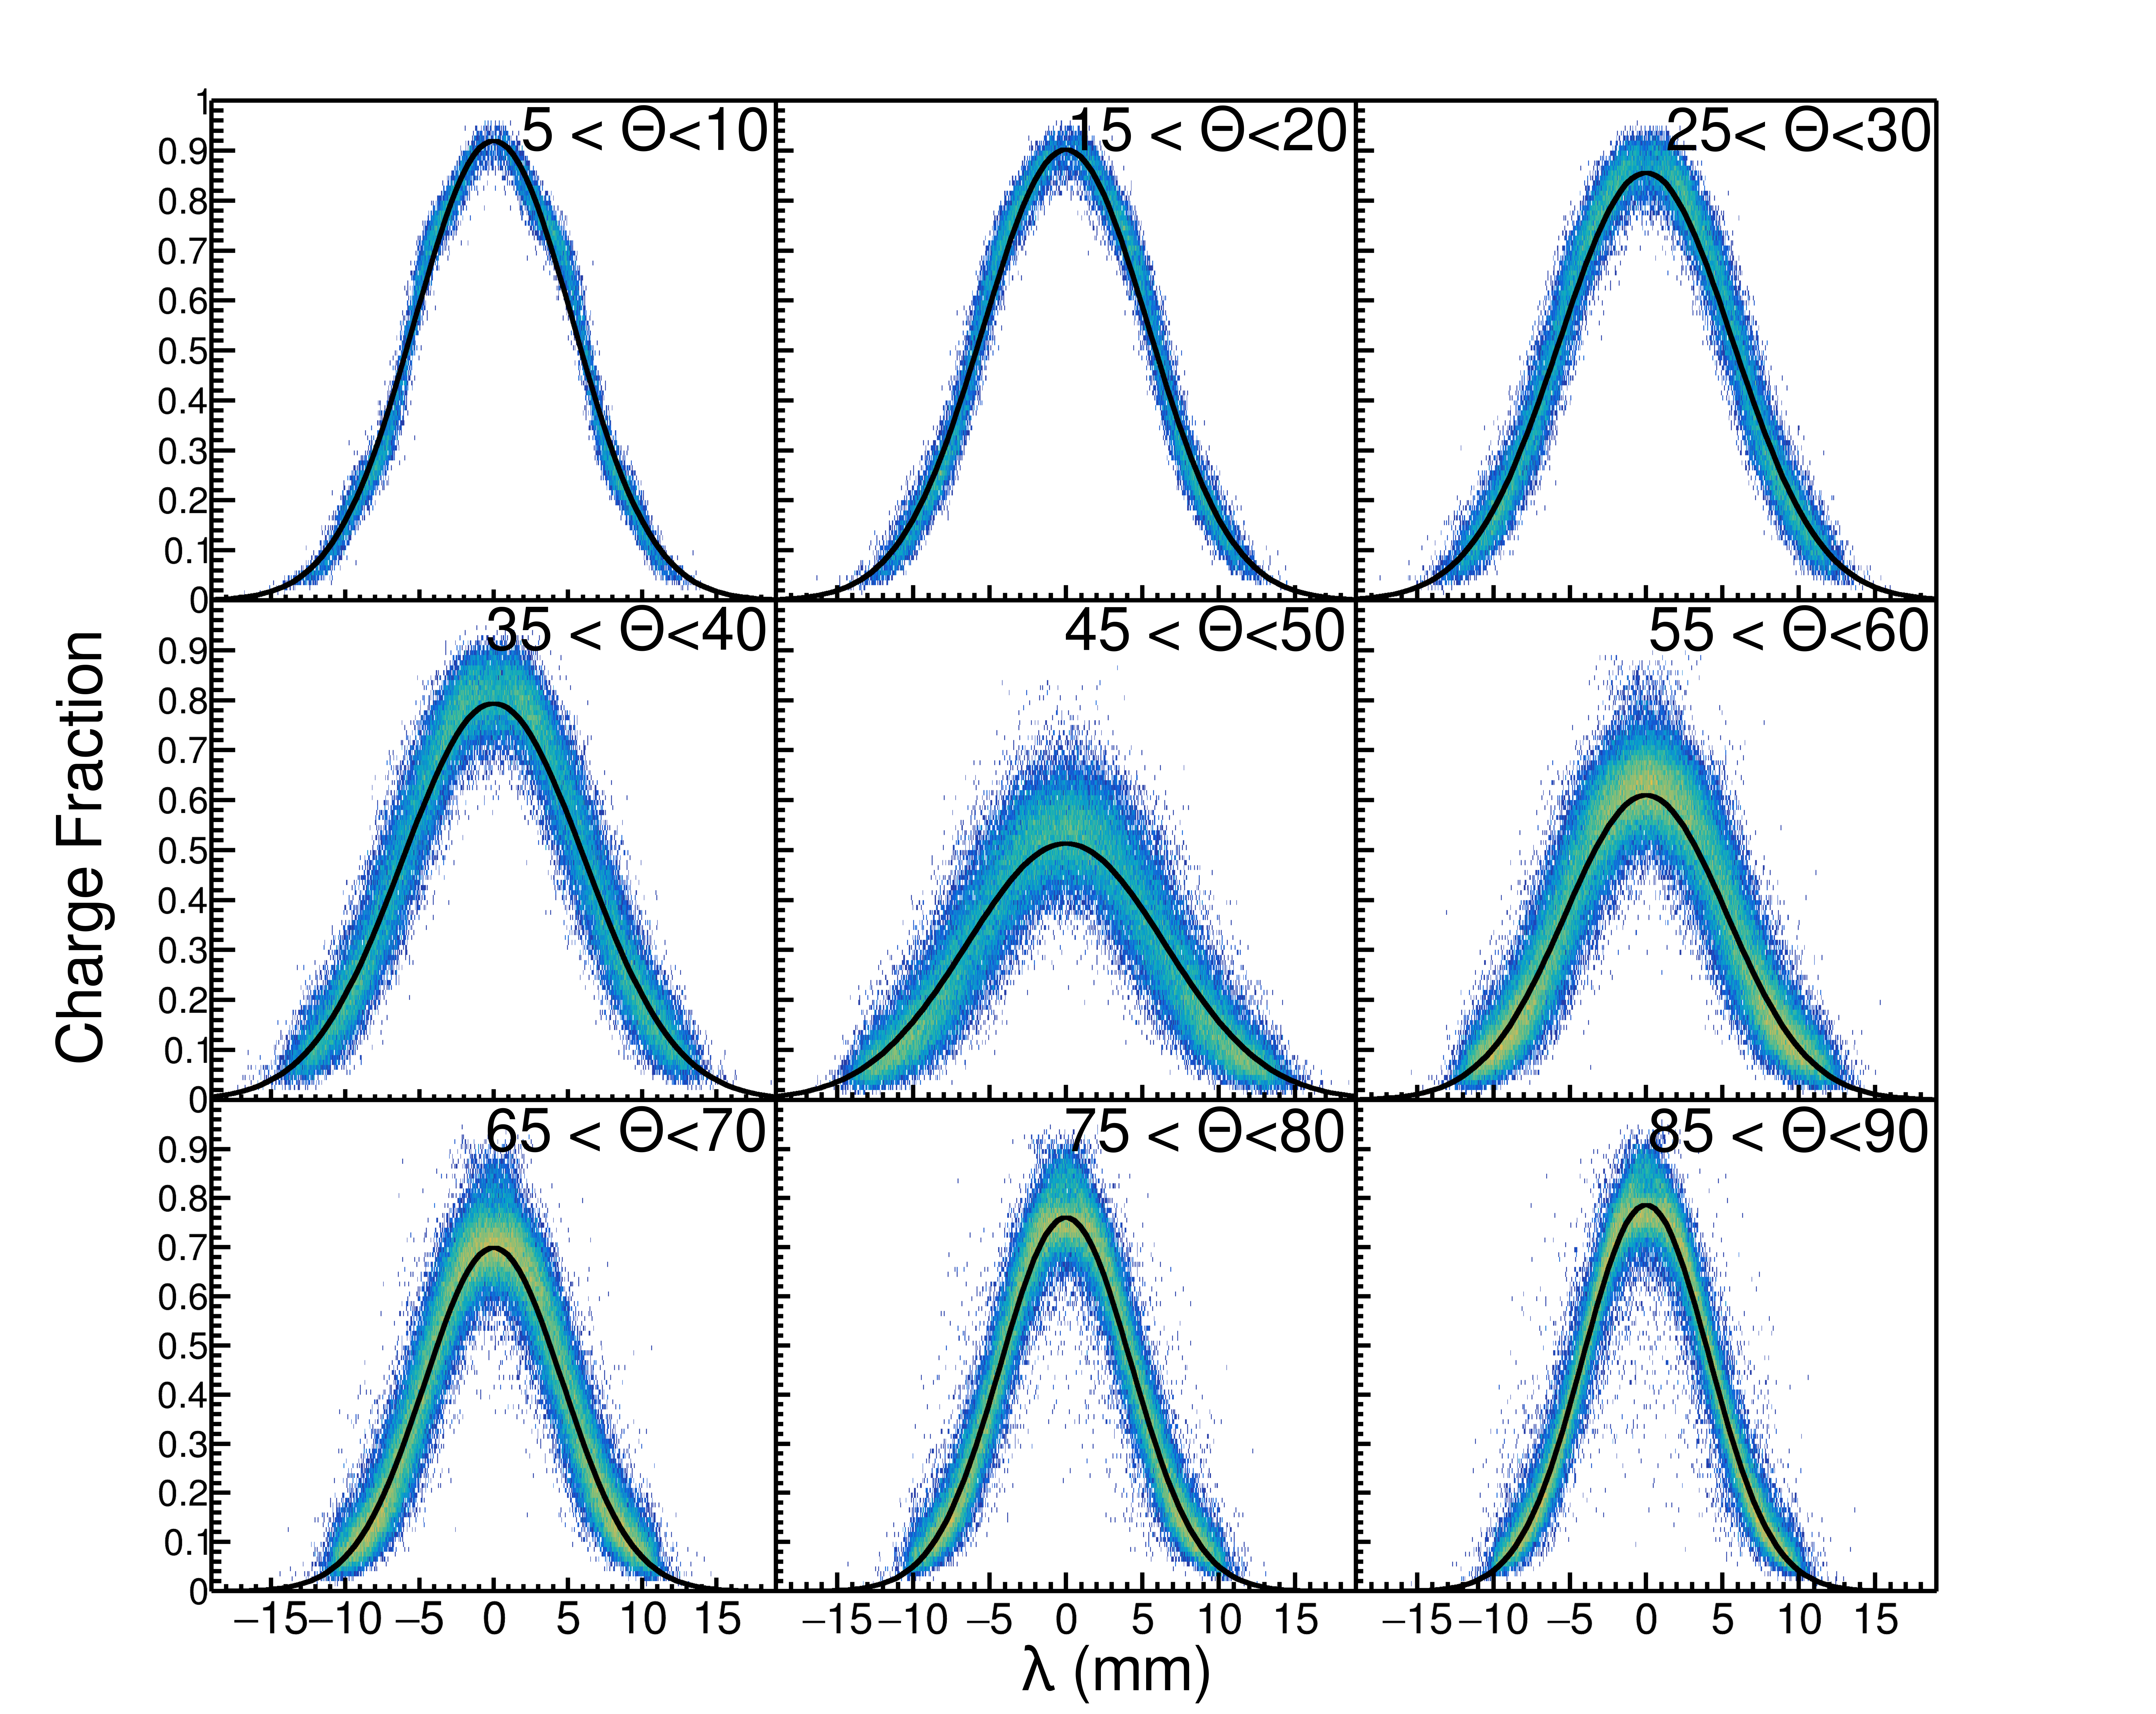
\includegraphics[width=\linewidth]{PRF_vsAngle}
\caption{Experimental pad response function as a function of the crossing angle $\theta$ }
\label{fig:prfangle}
\end{figure}


\begin{figure}[H]
\begin{overpic}[width=\linewidth]{normsigma}
\end{overpic}
\caption{Parameters $N_{0}$ and $\sigma$ as a function of the crossing angle $\theta$ with the $4^{th}$ order polynomial fits.}
\label{fig:normsigma}
\end{figure}

\begin{comment}
\begin{table}
\centering
 \begin{tabular}{||c c c c c c||} 
 \hline
 Coefficient & $c_0$ & $c_1$ & $c_2$ & $c_3$ & $c_4$ \\ [0.5ex] 
 \hline\hline
 $0 < \theta < 45$ & & & & &  \\ [.25ex]
 \hline
 $N_0$ & .897 & 5.766E-3 & -4.263E-4 & 7.444E-6 & 5.705E-8 \\ 
 \hline
 $\sigma$ & 5.496 & -3.920E-2 & 2.693E-3 & -5.208E-5 & 5.334E-7\\
 \hline
 $45 < \theta < 90$ & & & &  & \\ [.25ex]
 \hline	
 $N_0$ & 1.220 & -6.258E-2 & 1.608E-3 & -1.492E-5  & 4.654E-8 \\
 \hline
 $\sigma$ & 31.368 & -1.109 & 1.779E-2 & -1.336E-4 & 3.940E-7\\
 \hline
\end{tabular}
\caption{Coefficients of the $4_th$ order polynomial fit to the Gaussian parameters $N_0$ and $\sigma$. The polynomial form is given as $c_0 + c_1 x + c_2 x^2 + c_3 x^3 + c_4 x^4$}
\label{tb:coeff}
\end{table}
\end{comment}
 
Fit's were performed to the experimental data with  $5^{\circ}$ width bins from $0^{\circ} < \theta \leq 90^{\circ}$. The two parameters of the Gaussian fits are plotted versus $\theta$ in Figure \ref{fig:normsigma}; a $4^{th}$ order polynomial fit between these points allowed for interpolating between $\theta$.

\paragraph{Method of Desaturation}
We will use the term ``desaturation" for our process of correcting the charge values of the saturated pads. Figure \ref{fig:satpad} shows a typical situation of saturated signals. When an avalanche causes a large induced signal, the pads directly underneath collect the largest charge becoming saturated represented by $q_{2'}$ and $q_{3'}$. Pads further away experience smaller, non saturating charges represented by  $q_{1}$ and $q_{4}$. Though we don't know the saturated charge values, the distribution of all charges must follow the PRF which we have experimentally measured. From the clusters crossing angle, we can get the corresponding parameters for the PRF as described above in Figure \ref{fig:normsigma}.

We assume the distance of each pad to the track, $\lambda_i$ is fixed, this defines the fraction of charge each pad receives as defined by the $PRF(\lambda_i)$ function. 

A chi squared function, $\chi^2 = \sum_i \frac{(q_i^{obs} - q_i^{expect})^2}{q_i^{expect}}$, where $q_i^{obs}$ are the observed, non-saturated charges $q_{1}$ and $q_{4}$, and $q_i^{expect}$ are the expected charges observed; calculated as $ q_i^{expected} = Q\cdot PRF(\lambda_i)$. The charges, $q_{2'}$, $q_{3'}$, make up the unknown variable and are allowed to vary in the $\chi^2$ minimization but are added to make up the total expected charge Q. The minimum of the $\chi^2$ distribution gives best estimate for the saturated charge values on each pad. 


\begin{figure}[H]
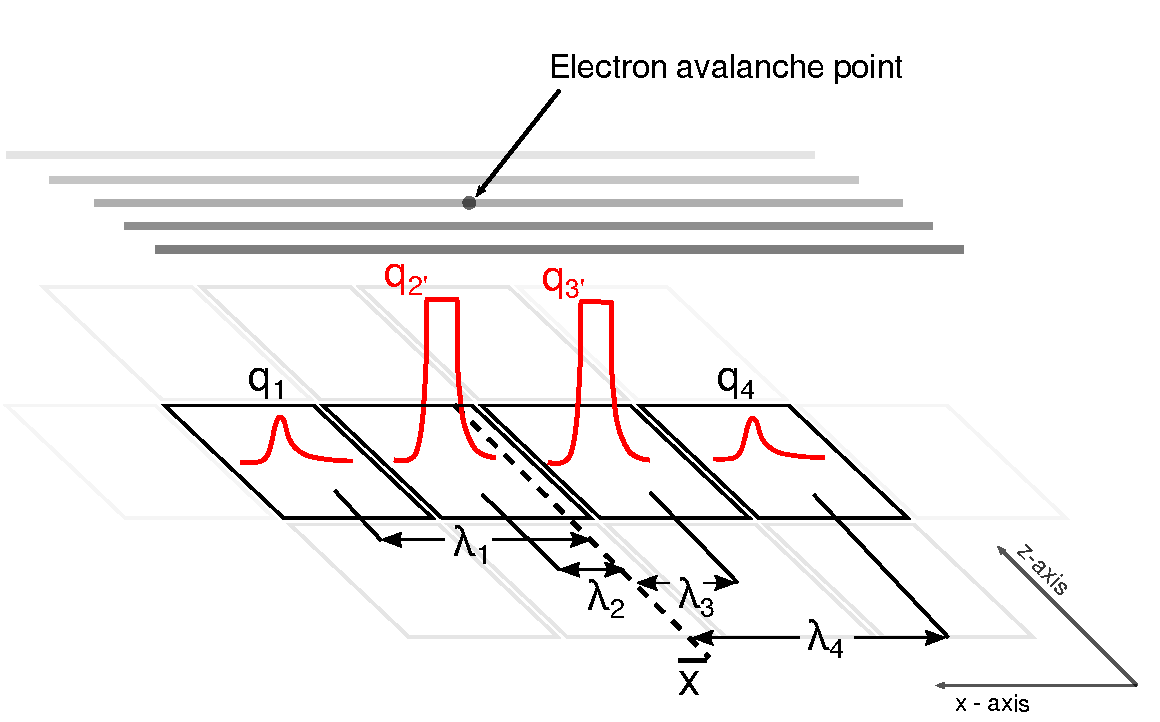
\includegraphics[width=\linewidth]{saturated_pads}
\caption{A typical case of a saturating event. The red pulses represent the time bucket signal for each collected charge. The pads directly underneath the avalanche point,$q_{2'}$ and $q_{3'}$, are saturated while pads farther away, $q_1$ and $q_4$ are not saturated.}
\label{fig:satpad}
\end{figure}

\section{Experimental data}
Two sets of data were used for the testing and validation of this method. A cocktail beam consisting of (p,d,t,${}^3He$,${}^4He$,${}^6Li$,${}^7Li$) light charged particles was injected into the TPC for calibration purposes, and tuned to two different ridgidity, $\beta\rho$, settings. The momentum resolution was approximately 1\%, as determined by the slits of the BigRIPS fragment separator of the Radioactive Isotope Beam Factory (RIBF) in RIKEN. A thick 21 mm thick aluminum target was inserted for part of the lower $\beta\rho$ setting, further reducing the energy of the beam for a third calibration point. 

In a typical cocktail event, one particle enters the TPC volume at a time and parallel to the pad plane, representing an ideal case for momentum and dE/dx determination; as it does not suffer from inefficiencies of high multiplicity events seen in the collision experimental data.  

\begin{figure}[H]
\includegraphics[width=\linewidth]{data.pdf}
\caption{Pad plane projection for a collision event in the TPC. Highlighted by red arrows are two regions of anode wires which had a reduced voltage of 1214 V. The voltage of the rest of the TPC anode wires are 1460 V. The reduction in voltage reduces the gain by a factor of about 10x. }
\label{fig:data}
\end{figure}

\begin{figure}[H]
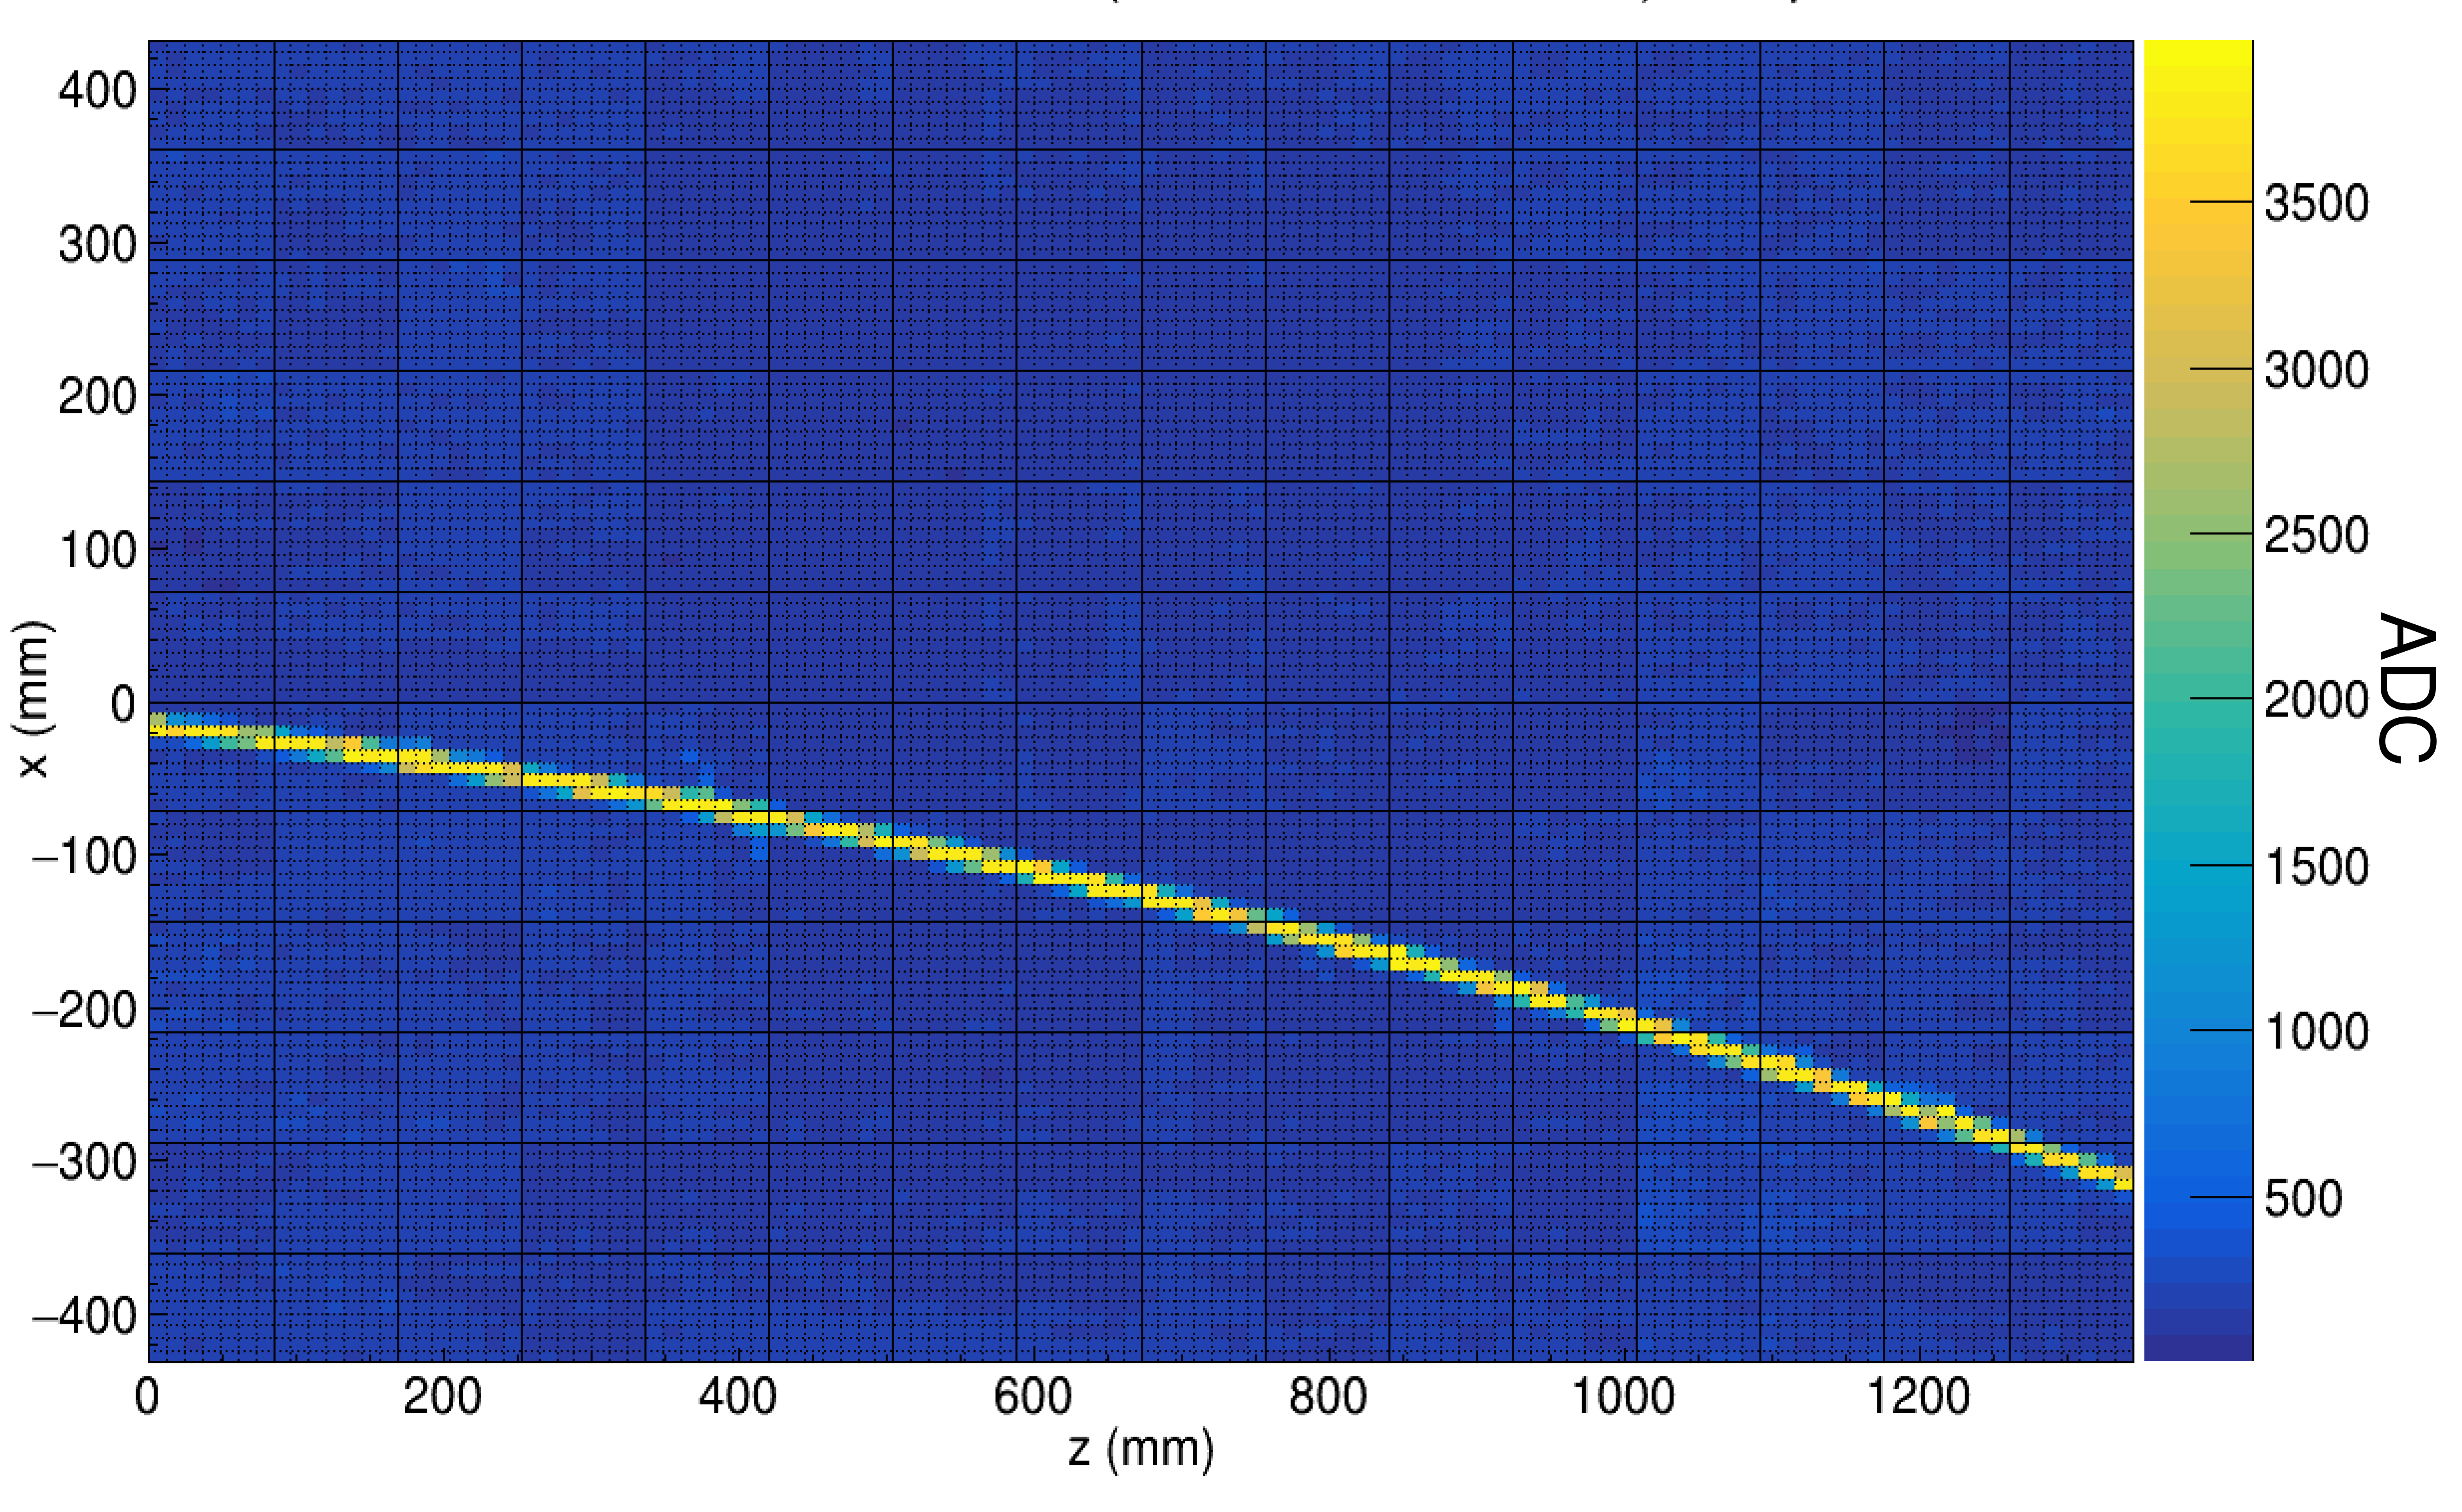
\includegraphics[width=\linewidth]{cocktail.png}
\caption{Pad plane projection for a cocktail event in the TPC.}
\label{fig:cocktail}
\end{figure}

The other type of data was the collision of a ${}^{132}$Sn beam onto a ${}^{124}$Sn target triggered on central nuclear collisions. Shown in Figure \ref{fig:data} is the typical pad plane response for a central nuclear collision. During the experiment the voltages of two anode sections (as indicated by red arrows in Figure \ref{fig:data}) were biased to 1214 V. The gain of these sections were also reduced by a factor of about 10 times, as compared with the other sections which were biased to 1460 V. We refer to the 1460 V region as high gain and the 1214 V region as low gain. 


\section{Results}
\paragraph{Low gain vs corrected high gain}

Tracks which saturate pads in the high gain region are not saturated in the low gain region; by comparing the dE/dx values of these two sections, we can directly measure the success of the high gain region's desaturation using the method described above.  

\begin{figure}[H]
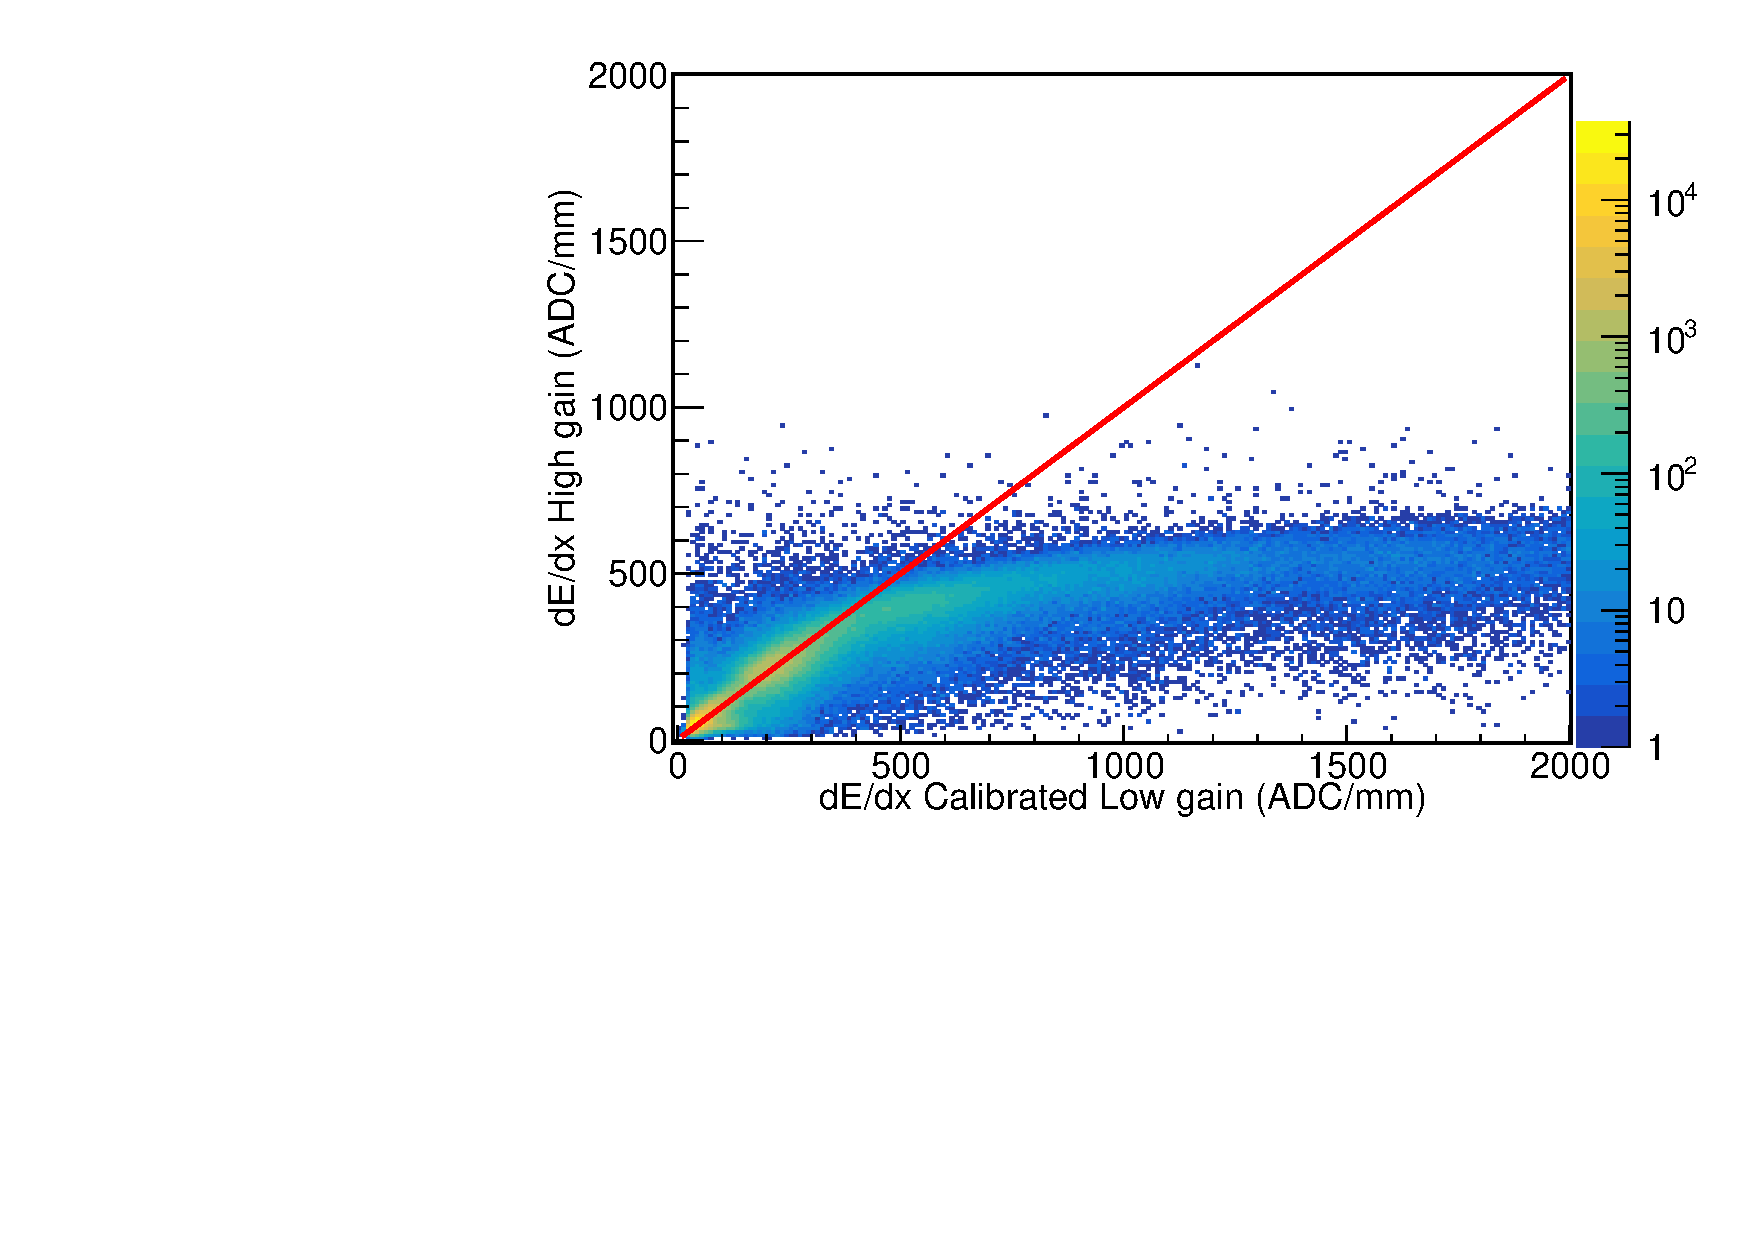
\includegraphics[width=\linewidth]{dedxcompare_nodesat}
\caption{The uncorrected high gain dE/dx vs low gain dE/dx collision data.  }
\label{fig:lowvshigh_raw}
\end{figure}
 
In Figure \ref{fig:lowvshigh_raw}, the effect of saturation can be seen in the high gain region for the uncorrected data. For signals below 400 ADC/mm the electronics are not saturated, and therefore the high and low gain sections agree. The data starts to saturate above 400 ADC/mm in the high gain channels eventually reaching a plateau; the low gain sections have not saturated and provide true dE/dx values.
 After applying the desaturation method, the correlation between the high and low gain sections is restored, as seen in Figure \ref{fig:lowvshigh_desat}. We believe the correction to at least about 2000 ADC/mm, increasing the dynamic range by a factor of 5.

\begin{figure}[H]
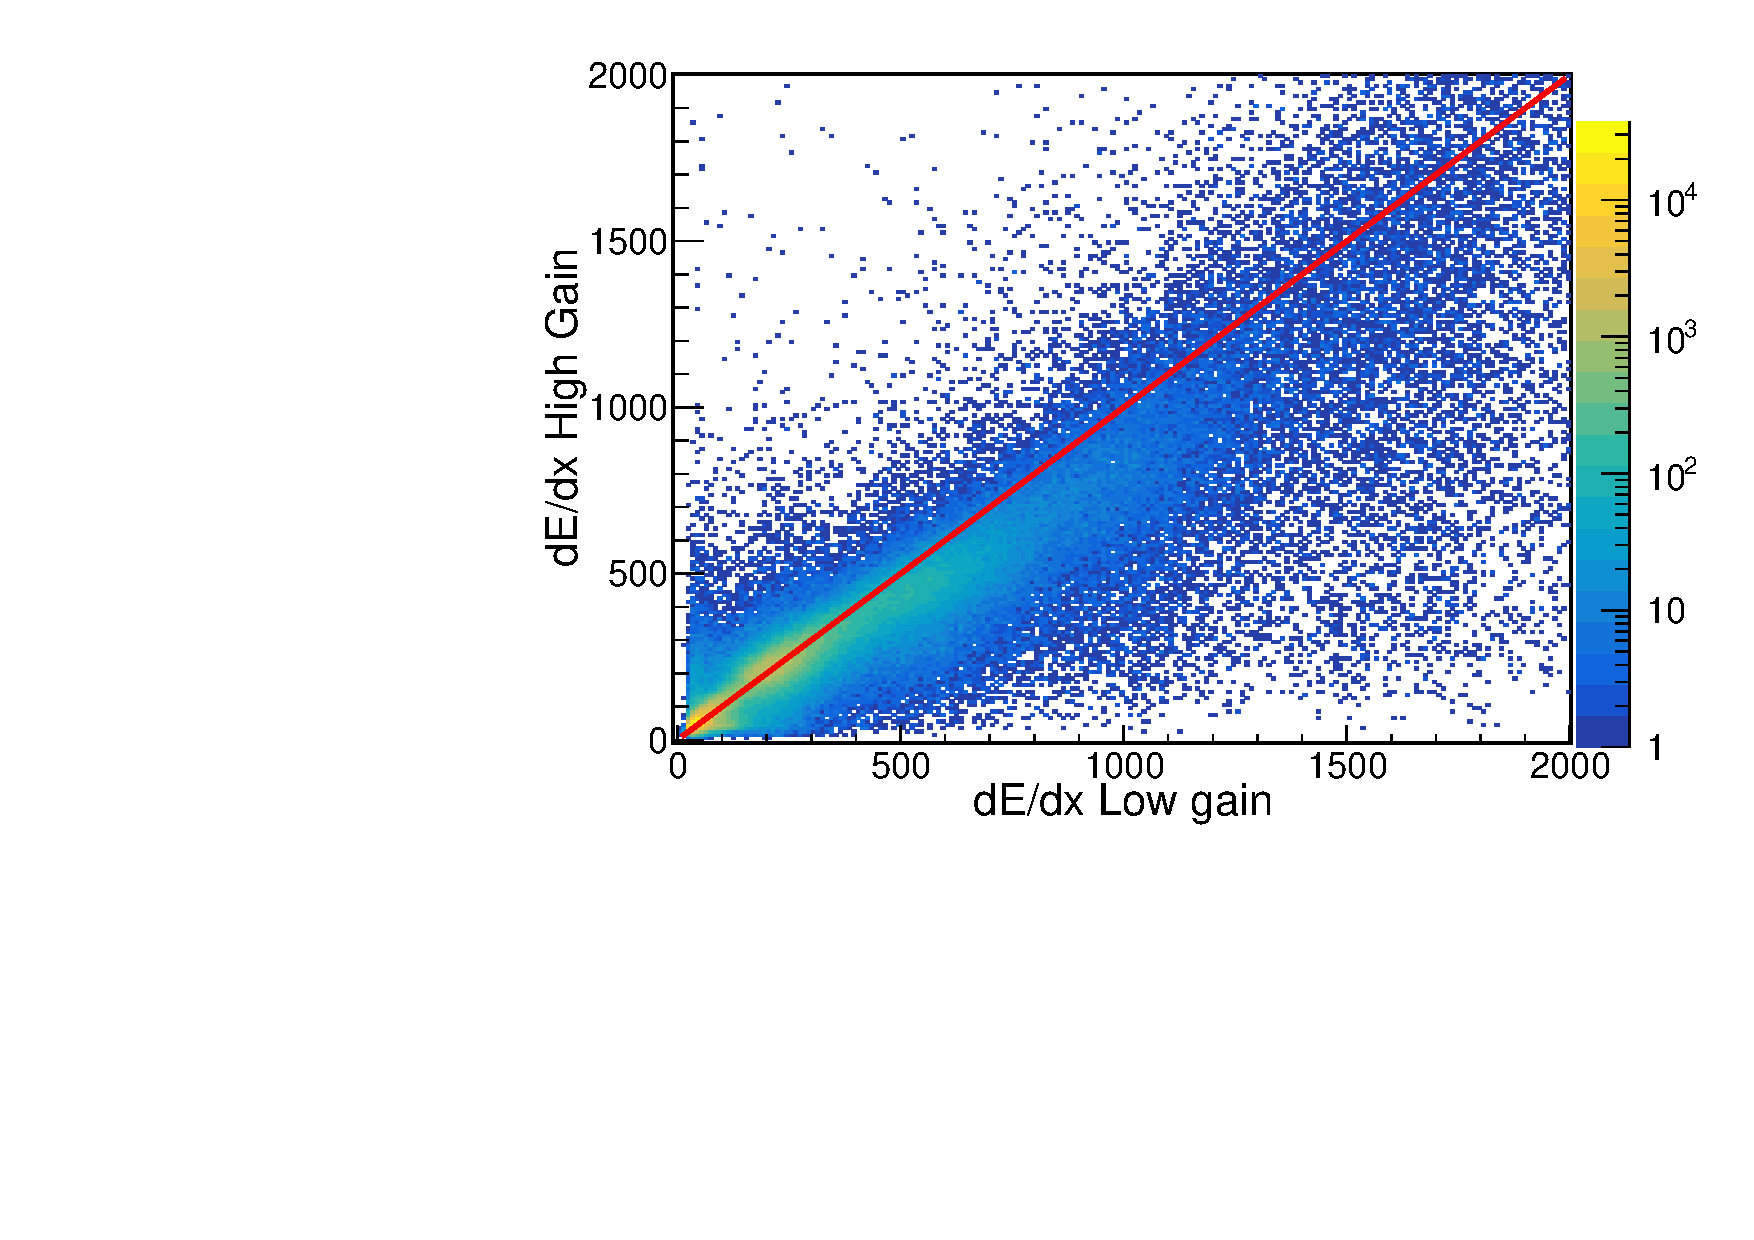
\includegraphics[width=\linewidth]{dedxcompare_new}
\caption{The corrected high gain dE/dx vs low gain dE/dx for collision data.  }
\label{fig:lowvshigh_desat}
\end{figure}

\paragraph{Particle Identification (PID)}


\begin{figure}[H]
\begin{overpic}[grid,width=\linewidth]{cocktail_combine.png}
\put(22,15){\contour{white}{\Large p} }
\put(27,20){\contour{white}{\Large d} }
\put(31,25){\contour{white}{\Large t} }
\put(30,31){\contour{white}{\large ${}^{3}$He} }
\put(33,35){\contour{white}{\large ${}^{4}$He} }
\put(60,26){\contour{white}{\large ${}^{6}$Li} }
\put(60,30){\contour{white}{\large ${}^{7}$Li} }

\end{overpic}
\caption{Uncorrected and corrected (desaturated) cocktail data.}
\label{fig:cocktail_raw}
\end{figure}

%\begin{figure}[H]
%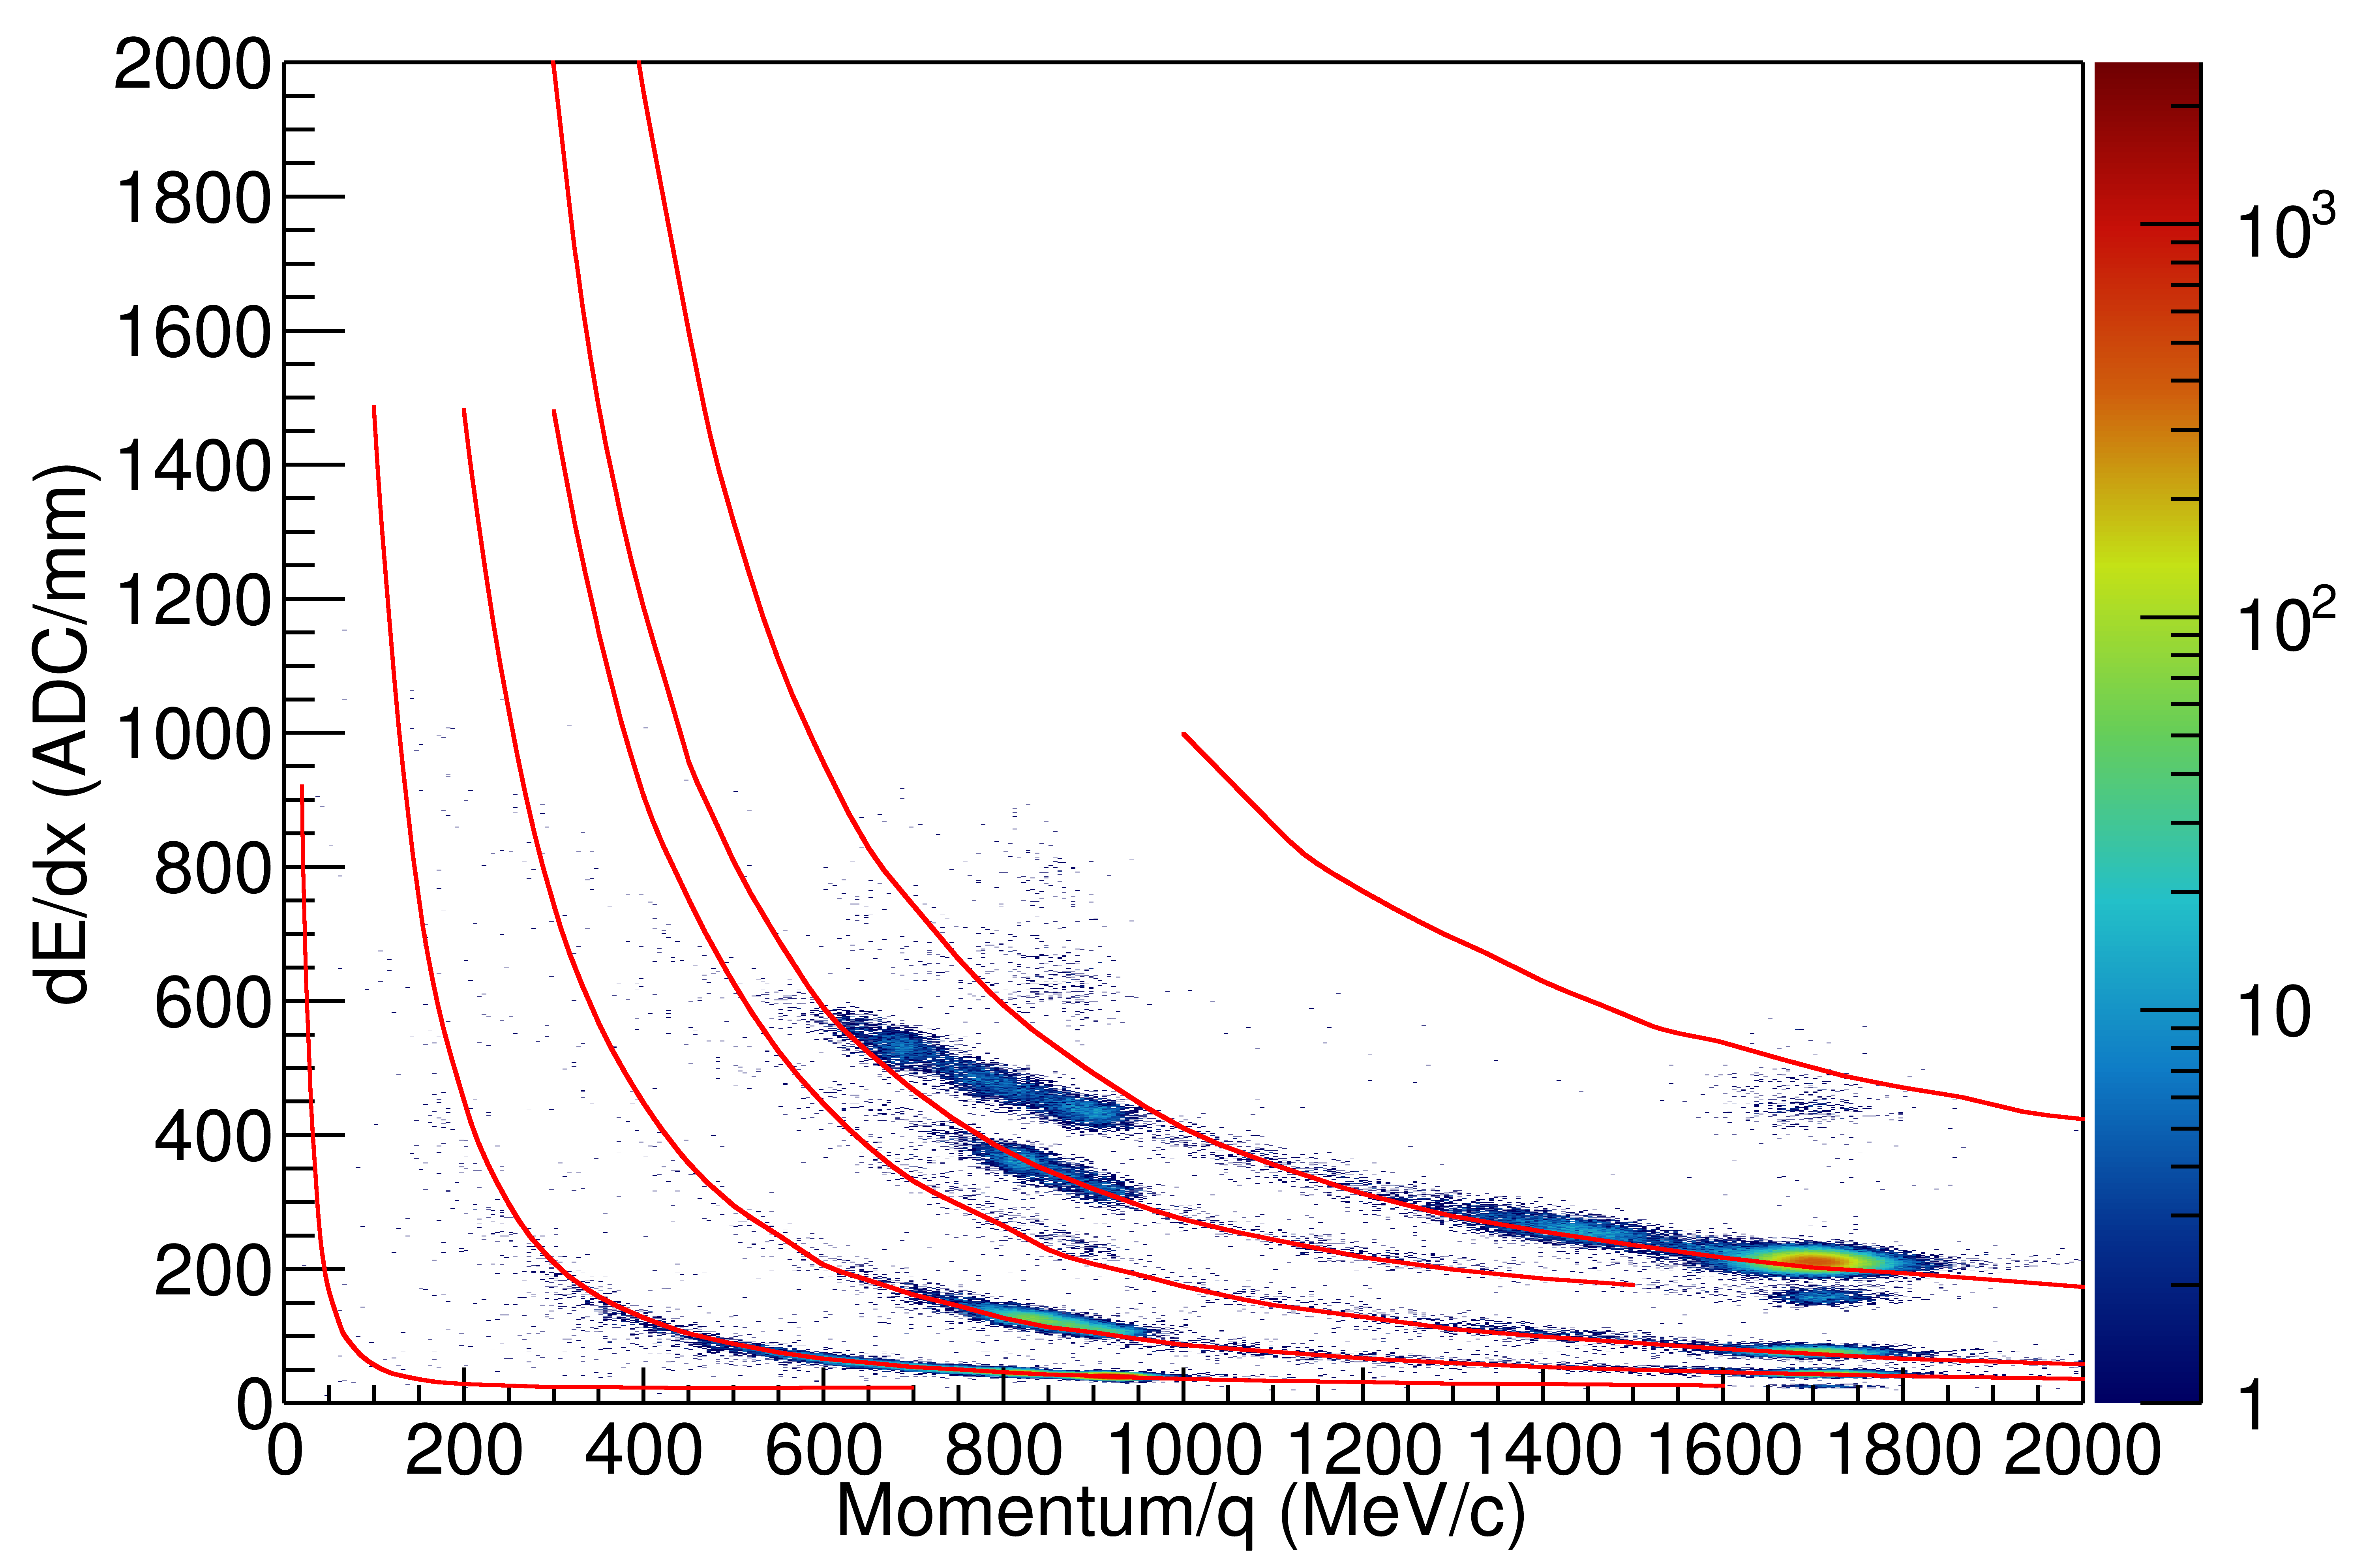
\includegraphics[width=\linewidth]{cocktail_sat.png}
%\caption{Uncorrected cocktail data.}
%\label{fig:cocktail_raw}
%\end{figure}

Comparing the low to high gain sections provides a direct measurement for determining the success of the desaturation technique, but the goal would be to improve the particle identification (PID). In the following PID plots the red lines represent the most probable energy loss as given by Geant4 straggling functions. A linear calibration was performed to convert keV in Geant4 to ADC in the experiment given by $\frac{ADC}{mm} = 20. \frac{keV}{cm}$.


There are pronounced PID lines of several particle species in both the uncorrected and corrected cocktail beam PID in figures \ref{fig:cocktail_raw} and \ref{fig:cocktail_desat}. Three ovals around a momentum of 1700 and two near 900 MeV/c/Z correspond to the three B$\rho$ settings injected into the TPC. The tails of the PID lines resulting from the particle losing its initial energy, passing through the walls and other materials outside the main detector volume; therefore lowering their initial momentum. 

The uncorrected data in Figure \ref{fig:cocktail_raw} shows the effects of saturation; the PID lines deviate from their theoretical expectations starting around 400 ADC/mm eventually reaching a plateau. After applying the desaturation technique, we see a large improvement; most notably the He and Li particles, which suffer the most from saturation. A more subtle improvement of the lighter particles, (p,d,t), can also be seen in the PID lines at lower momentum.

\begin{comment}
\begin{figure}[H]	
\begin{overpic}[width=\linewidth]{cocktail_desat.png}
\put(22,15){\contour{white}{\Large p} }
\put(27,20){\contour{white}{\Large d} }
\put(31,25){\contour{white}{\Large t} }
\put(30,31){\contour{white}{\large ${}^{3}$He} }
\put(34,35){\contour{white}{\large ${}^{4}$He} }
\put(60,26){\contour{white}{\large ${}^{6}$Li} }
\put(60,30){\contour{white}{\large ${}^{7}$Li} }

\end{overpic}
\caption{Corrected (desaturated) cocktail data.}
\label{fig:cocktail_desat}
\end{figure}
\end{comment}

%\begin{figure}[H]
%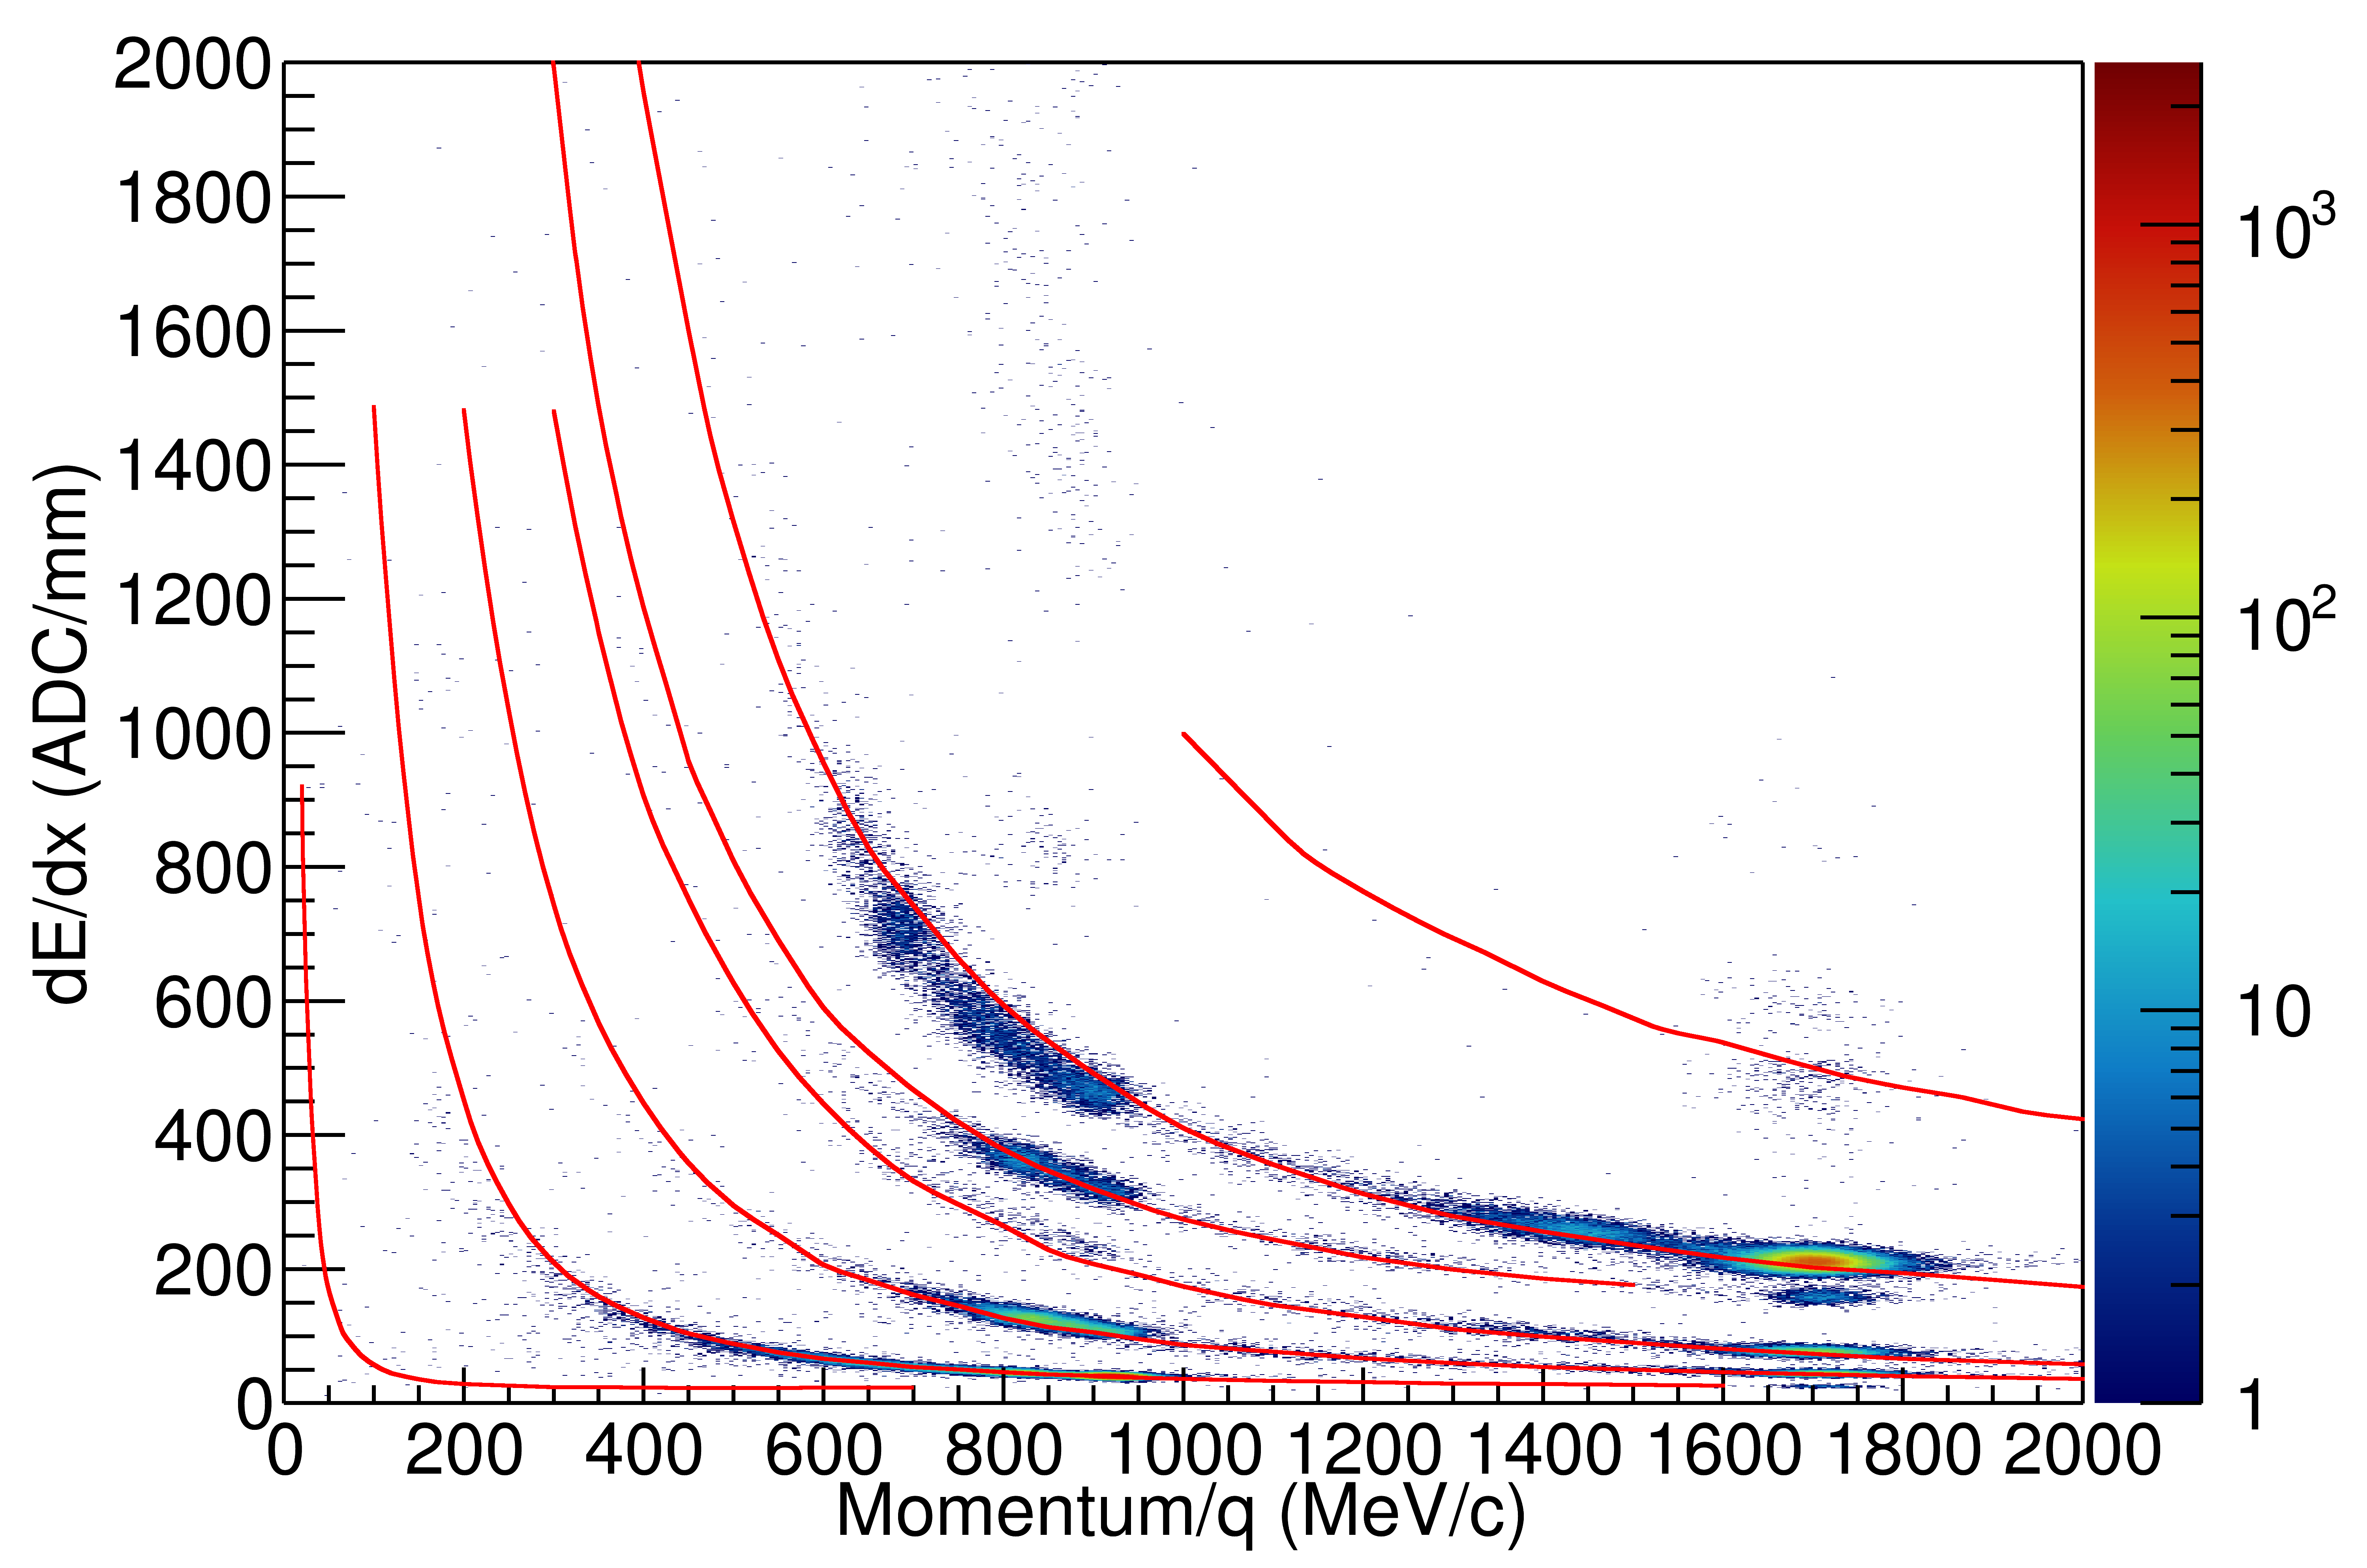
\includegraphics[width=\linewidth]{cocktail_desat.png}
%\caption{Corrected (desaturated) cocktail data.}
%\label{fig:cocktail_desat}
%\end{figure}


 
Looking at the collision data, in figures $\ref{fig:data_raw}$ and $\ref{fig:data_desat}$, we also see a similar result. The collision data PID suffers from more background and inefficiencies than the cocktail beam; nevertheless we can see a similar improvement in the PID lines when comparing the uncorrected to after the desaturation has been applied. Notably the separation of particle species at lower momenta and the separation of the Li species into ${}^{6}$Li and ${}^{7}$Li, whereas there was little to no separation before. 

\begin{figure}[H]	
\begin{overpic}[width=\linewidth]{data_combine.png}
\put(22,15){\contour{white}{\Large p} }
\put(27,20){\contour{white}{\Large d} }
\put(31,25){\contour{white}{\Large t} }
\put(30,31){\contour{white}{\large ${}^{3}$He} }
\put(34,35){\contour{white}{\large ${}^{4}$He} }
\put(60,26){\contour{white}{\large ${}^{6}$Li} }
\put(60,30){\contour{white}{\large ${}^{7}$Li} }

\end{overpic}
\caption{Uncorrected and corrected (desaturated) collision data at polar angles of $\theta < 40^{\circ} and -80^{\circ} < \phi < 80^{\circ}$}
\label{fig:data_raw}
\end{figure}

%\begin{figure}[H]
%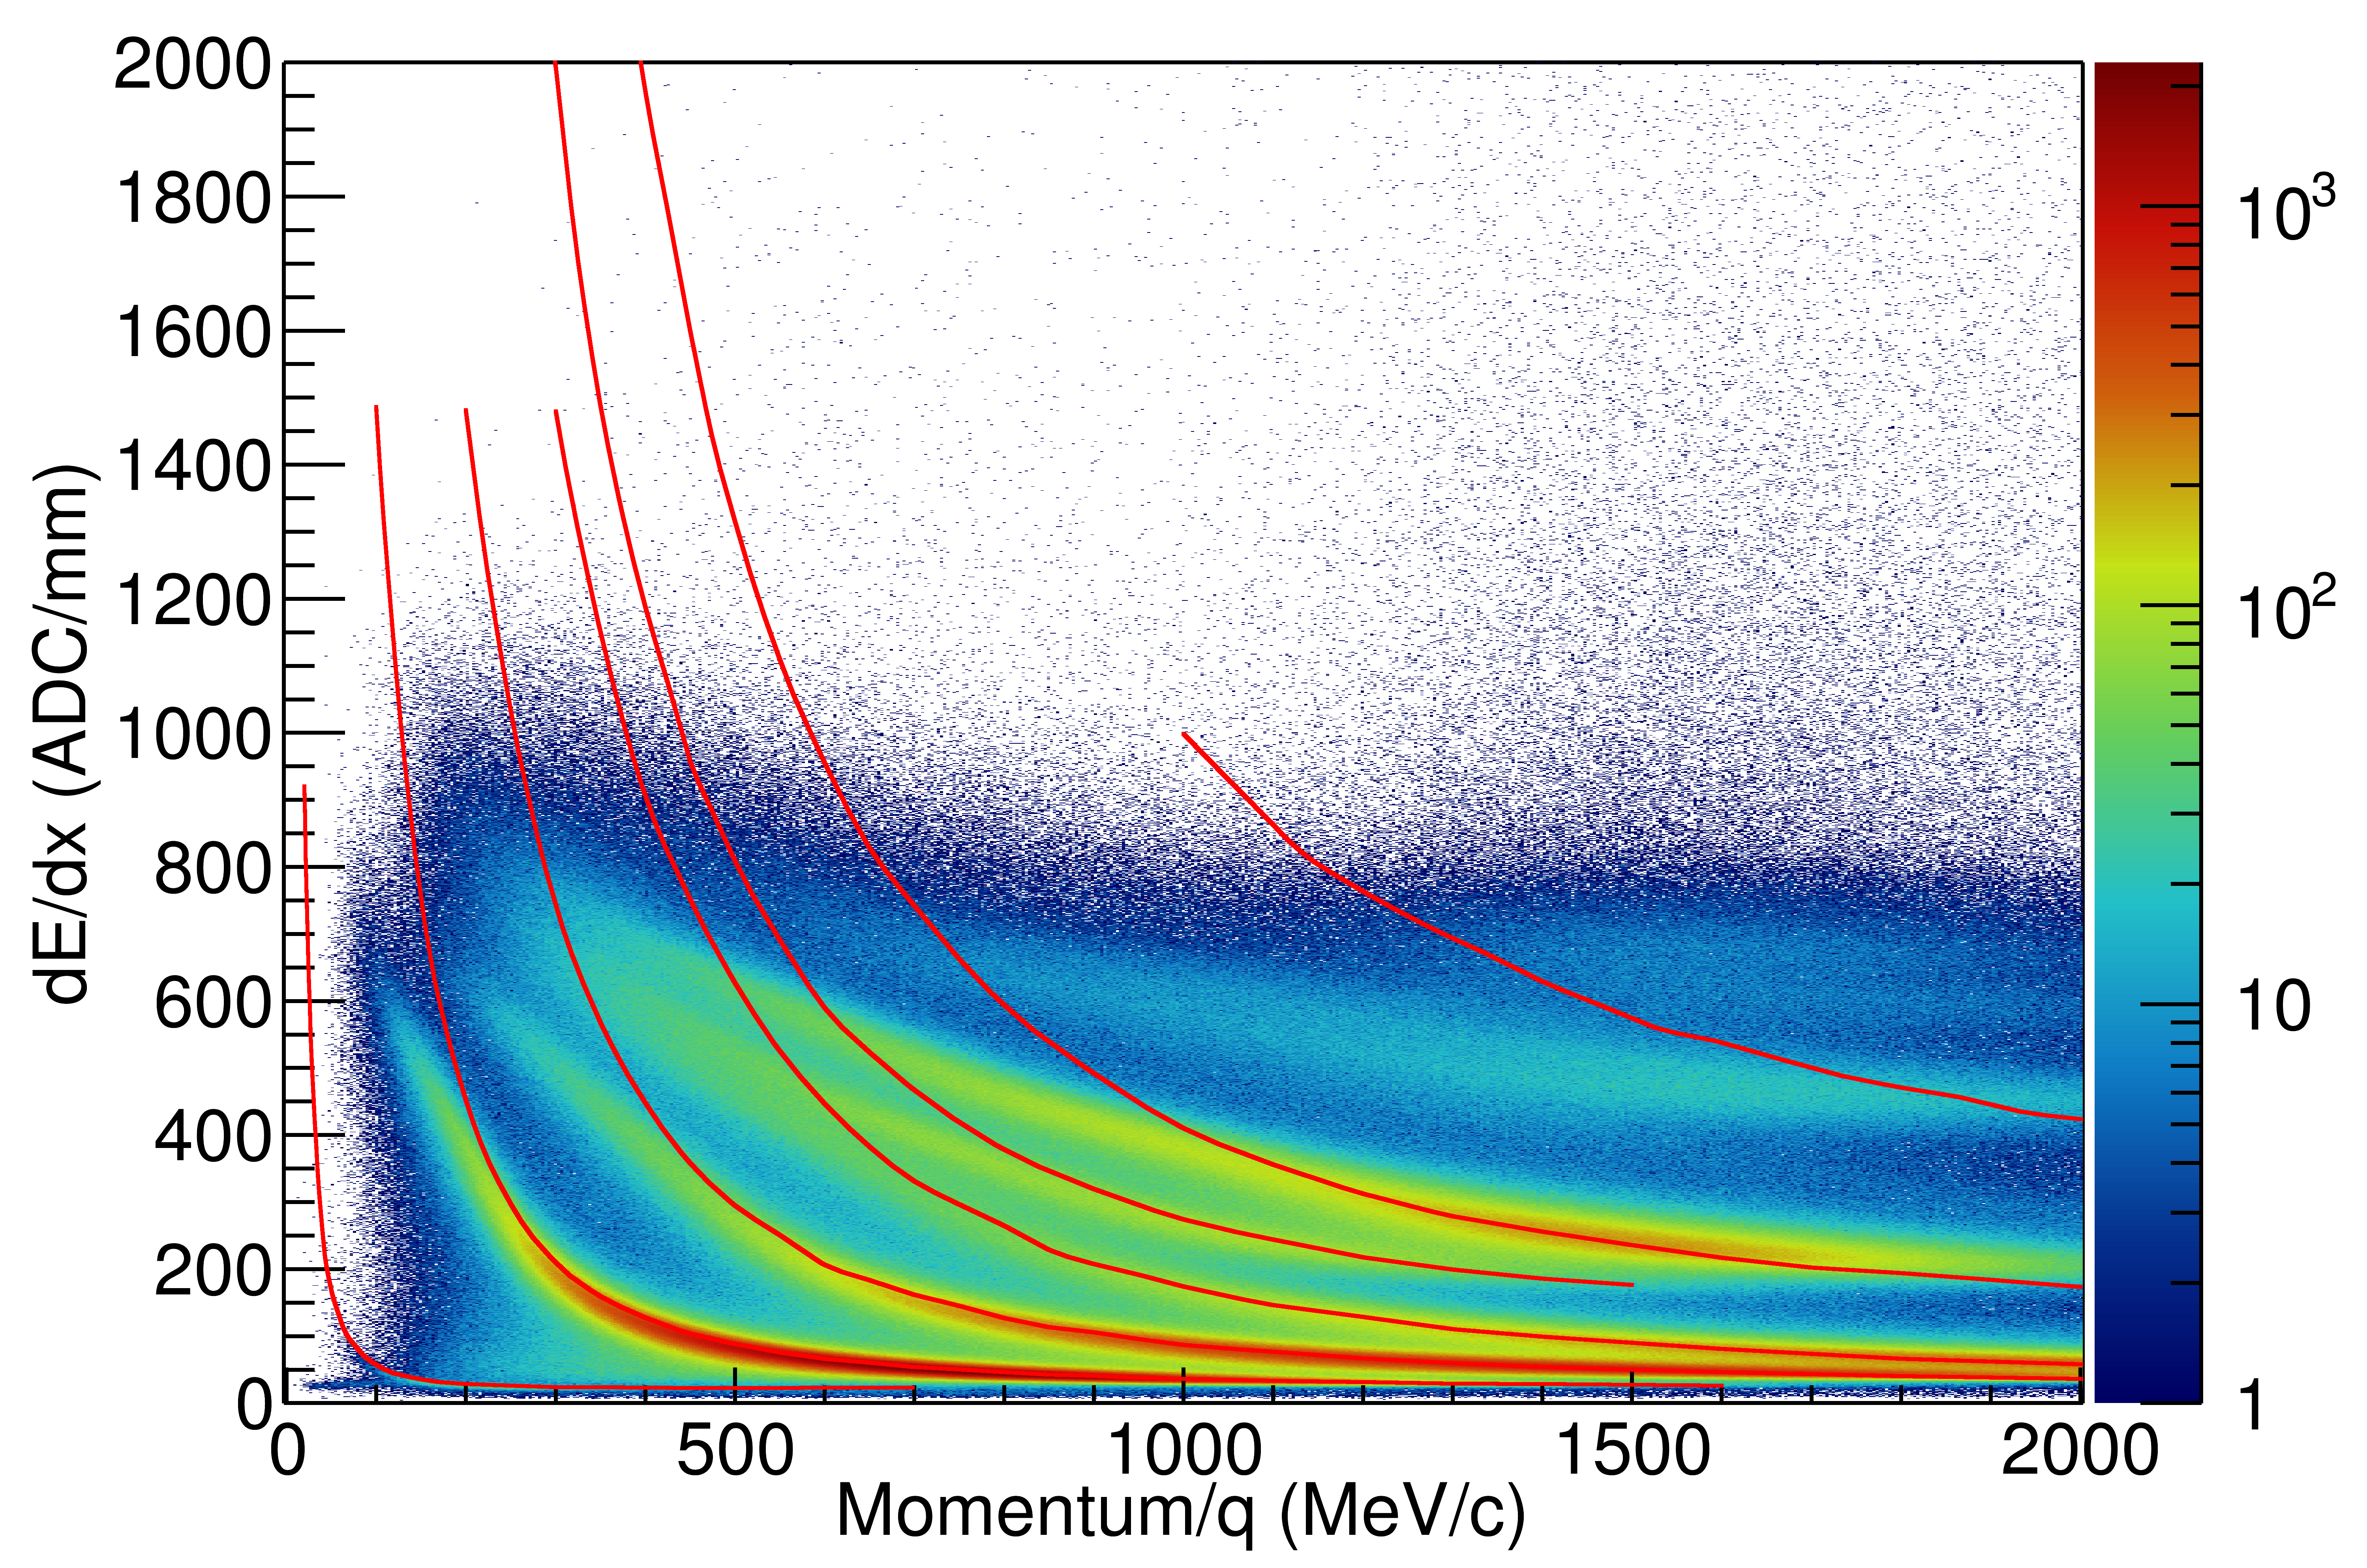
\includegraphics[width=\linewidth]{data_sat.png}
%\caption{Uncorrected collision data.}
%\label{fig:data_raw}
%\end{figure}

\begin{comment}
\begin{figure}[H]	
\begin{overpic}[width=\linewidth]{data_desat.png}
\put(22,15){\contour{white}{\Large p} }
\put(27,20){\contour{white}{\Large d} }
\put(31,25){\contour{white}{\Large t} }
\put(30,31){\contour{white}{\large ${}^{3}$He} }
\put(34,35){\contour{white}{\large ${}^{4}$He} }
\put(60,26){\contour{white}{\large ${}^{6}$Li} }
\put(60,30){\contour{white}{\large ${}^{7}$Li} }

\end{overpic}
\caption{Corrected (desaturated) collision data. $\theta < 40^{\circ} and -80^{\circ} < \phi < 80^{\circ}$}
\label{fig:data_desat}
\end{figure}
\end{comment}

%\begin{figure}[H]
%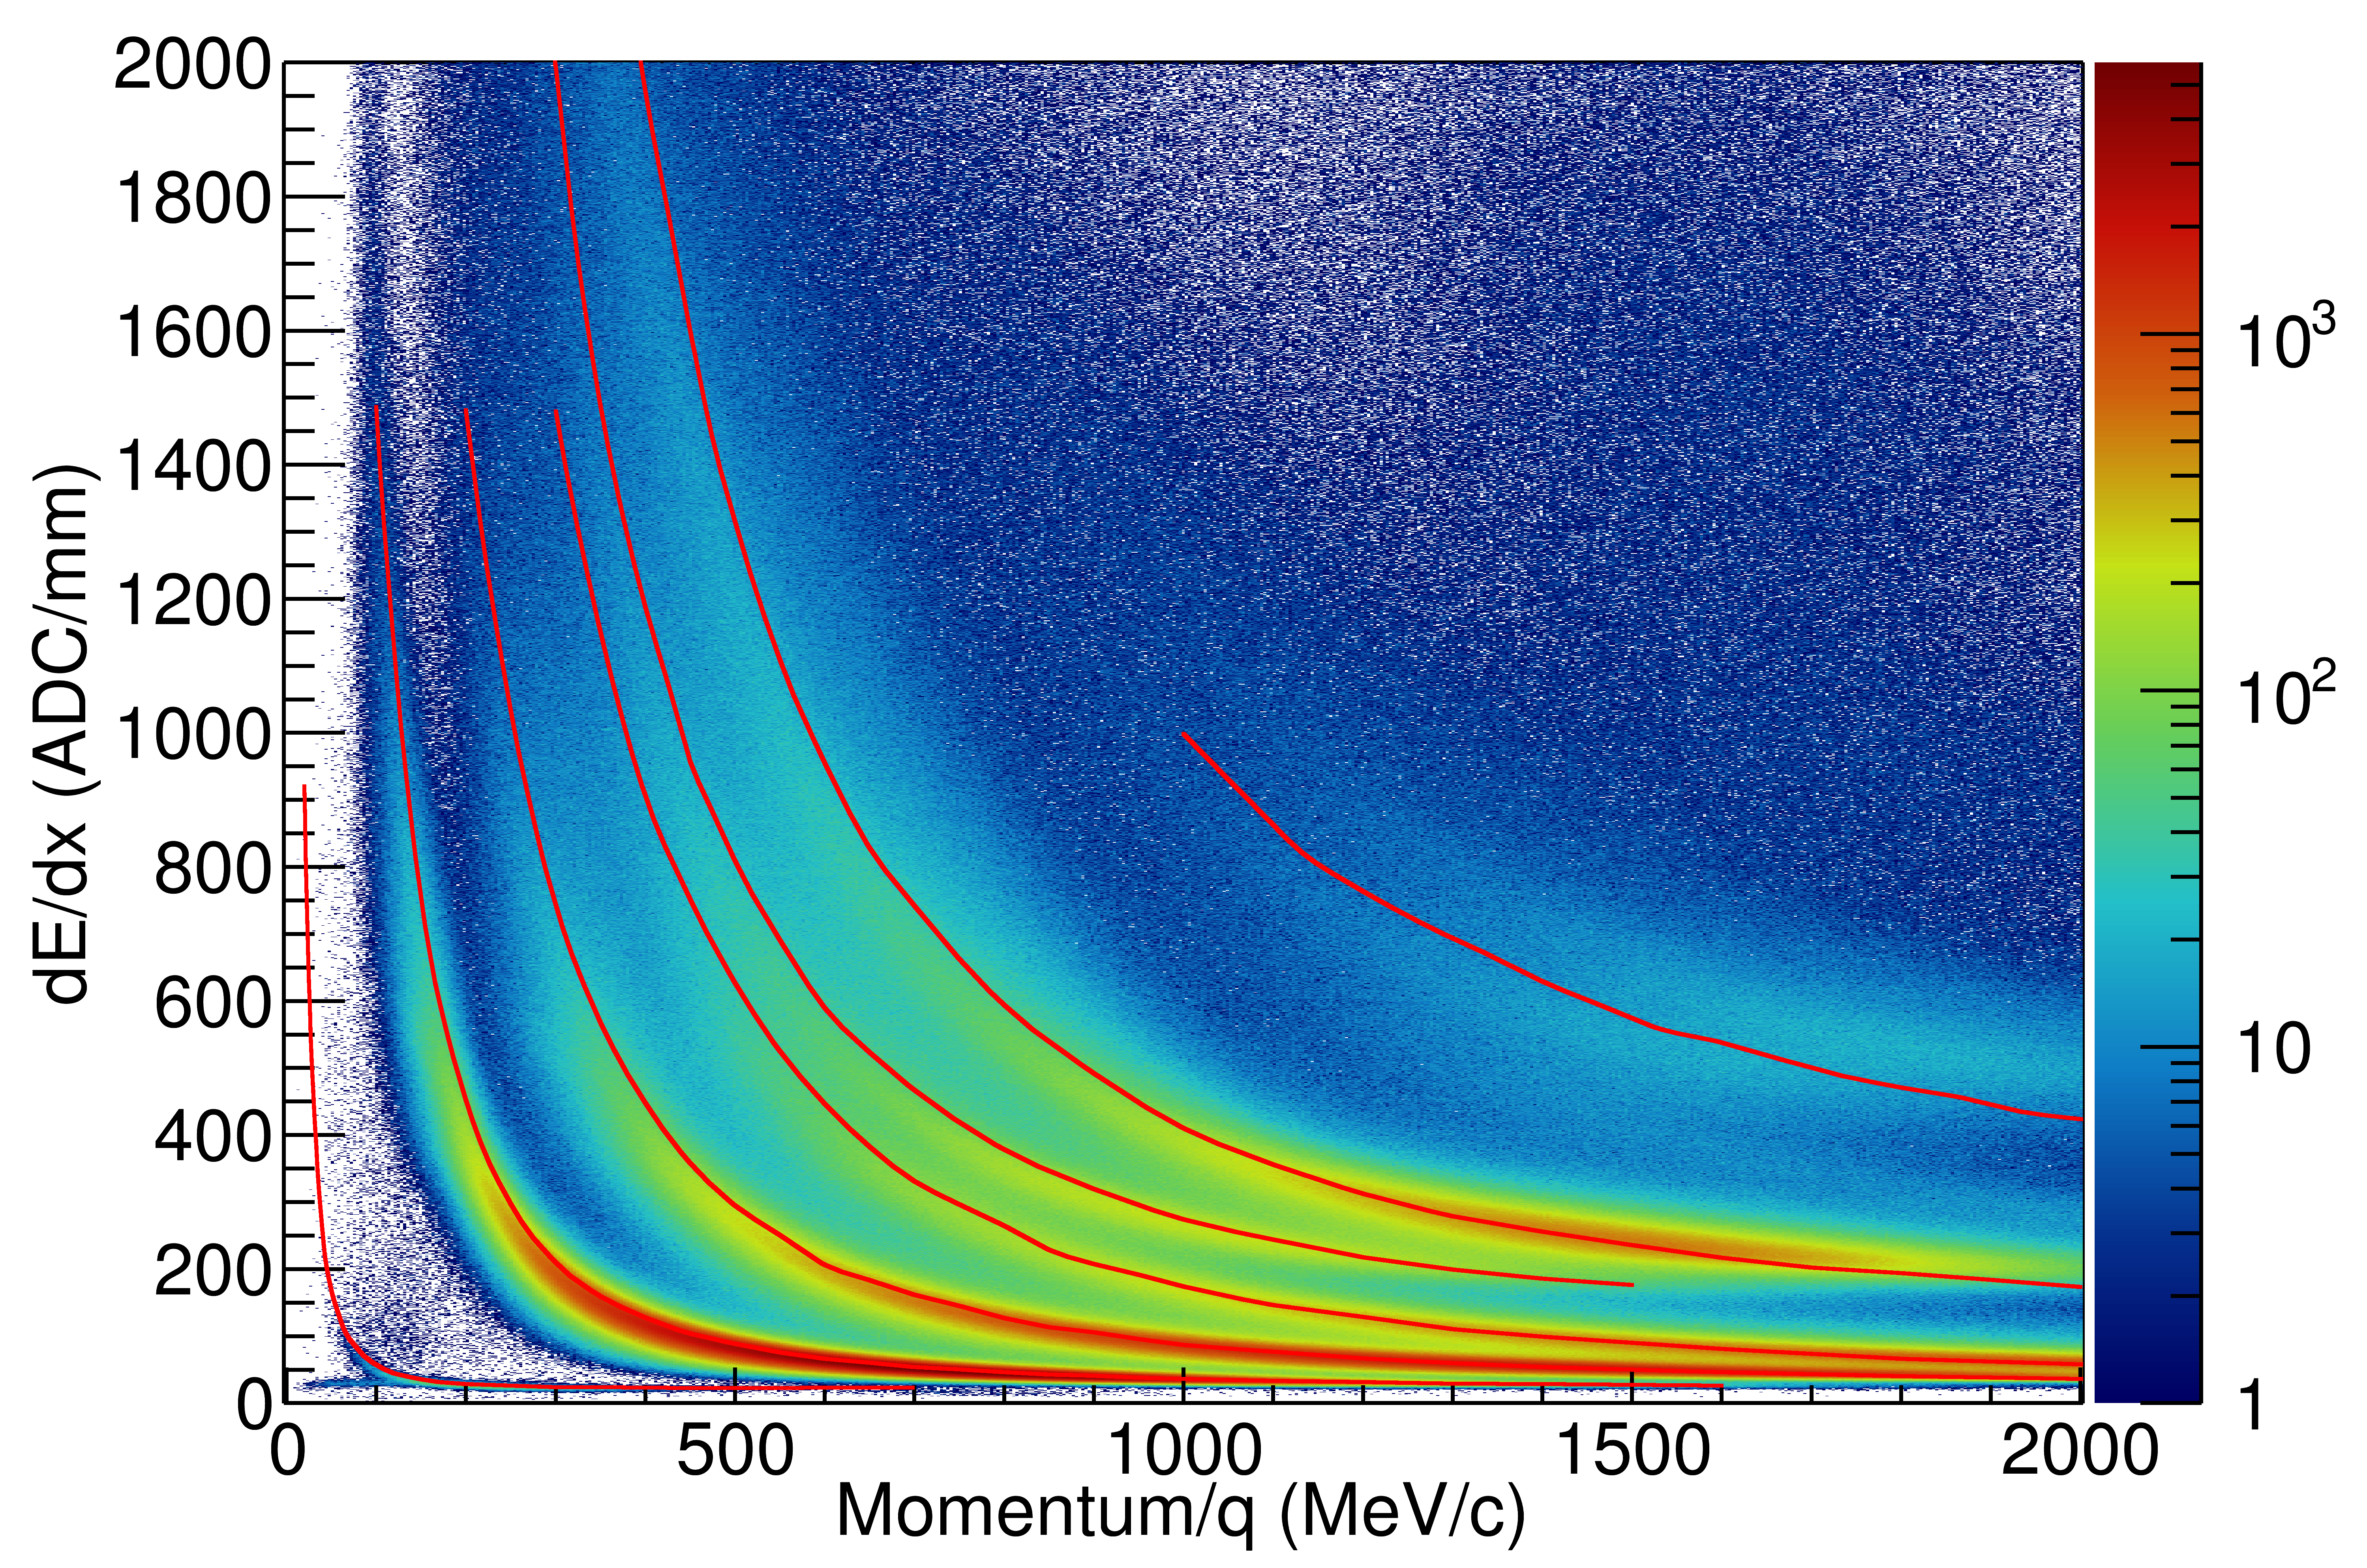
\includegraphics[width=\linewidth]{data_desat.png}
%\caption{Corrected (desaturated) collision data.}
%\label{fig:data_desat}
%\end{figure}


\section{Conclusion}

The saturation  of the electronics reduces dE/dx resolution and even the maximum charge observable inside of a TPC.  We have shown that some of the saturation is recoverable. Since the Pad Response Function of the TPC is fixed by the anode wire geometries, an experimental PRF can be calculated from the unsaturated experimental data. The charge distribution resulting from an avalanche on a wire must follow this PRF even if the electronics of some channels directly under the avalanche are saturated. The pads further away are not saturated; by using these unsaturated pads we perform applying a $\chi^2$  fit the unknown saturated pads to the known PRF. 

Looking at the PID lines, and also making a direct comparison to some low gain sections of the TPC, we were able to extend the dynamic range of our electronics by a factor of about 5 times. This improved PID will allow for us to extend the momentum distributions of all species to lower momenta than what was previously available. 

\section{Acknowledgments}
This work was supported by the U.S. Department of Energy under Grant Nos.  DE-SC0004835,  DE-SC0014530, DE-NA0002923,  US  National Science Foundation Grant  No.  PHY-1565546, the  Japanese  MEXT  KAKENHI(Grant-in-Aid  for  Scientific  Research  on  Innovative  Areas)  grant  No. 24105004, and Polish National Science Center (NCN), under contract Nos. UMO-2013/09/B/ST2/04064 and UMO-2013/10/M/ST2/00624. The computing resources for analyzing the data was provided by the HOKUSAI-GreatWave system at RIKEN and the MSU HPCC. 

\section*{References}

\bibliography{mybibfile}

\end{document}